\chapter{Case Study: Impacts of climate change on competing forest ecosystem services}
\label{ch:caseStudyDeschutes}
To demonstrate the application of the hypervolume indicators and the proposed pairwise objective metric to the analysis of conflict in multi-objective systems, we perform a case study on forest management in the Deschutes National Forest. We compare the conflict among ecosystem services in three multi-objective systems: one in which climate change is ignored, one in which climate change is predicted to be mild, and one in which it is predicted to be severe. For each climate change scenario, we solve a multi-objective mathematical program that optimizes ecosystem service achievement. The model aims to minimize fire hazard and sediment delivery while maximizing habitat for the northern spotted owl. In the coming sections we describe the study area and the importance of each of these ecosystem services. We then formally define the mathematical program solved for each climate change scenario, describe the climate scenarios considered, and finally present and discuss the results.

\section{Study area and selection of ecosystem services}
\label{sec:studyArea}
%To provide context for the selection of ecosystem services for the model, we first describe the area in which the case study was conducted.
Our study area is the Drink Planning Area. It consists of 7056 ha of federally owned forest land on the east slopes of the Cascade Mountain Range located within the Deschutes National Forest. See Figure \ref{fig:drinkOverview}. Having never undergone logging or treatment, the Drink contains large areas of old growth forest. The large swaths of old growth forest in the Drink make it prime habitat for the northern spotted owl (NSO) (\textit{Strix occidentalis caurina}, Figure \ref{fig:nso}), an iconic % (albeit controversial \cite{simberloff1998flagships}) 
inhabitant of Pacific Northwest forests that is listed as a federally threatened species \cite{congress1973endangered}. However, the same old growth conditions that render the area suitable habitat for the NSO also render it susceptible to high-severity wildfires. Such a wildfire would put at risk the NSO's habitat \cite{courtney2004scientific} as well as one of the Drink's other notable features - the municipal watershed for the cities of Bend, OR and Sisters, OR. Wildfires pose a threat to these cities' water supply, because they can cause soil water repellency, surface runoff, and debris torrents \cite{ice2004effects} which degrade watershed quality.

\begin{figure}[ht]
\centering
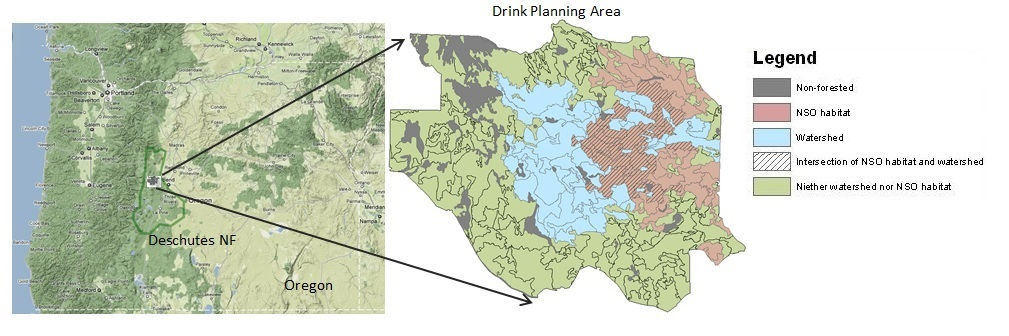
\includegraphics[width=.9\textwidth]{../images/Drink_Overview}
\caption[Overview of the study system, the Drink Planning Area]{Overview of the study system, the Drink Planning Area, consisting of 7056 ha in the Deschutes National Forest. The Drink Area contains old growth forest that make it suitable habitat for the northern spotted owl. It also houses the municipal watershed for Bend, OR and Sisters, OR.}
\label{fig:drinkOverview}
\end{figure}

\begin{figure}
\centering
\caption[Northern spotted owl]{The northern spotted owl is a threatened species whose habitat includes forests in the Pacific Northwest, including the Drink Area.}
\label{fig:nso}
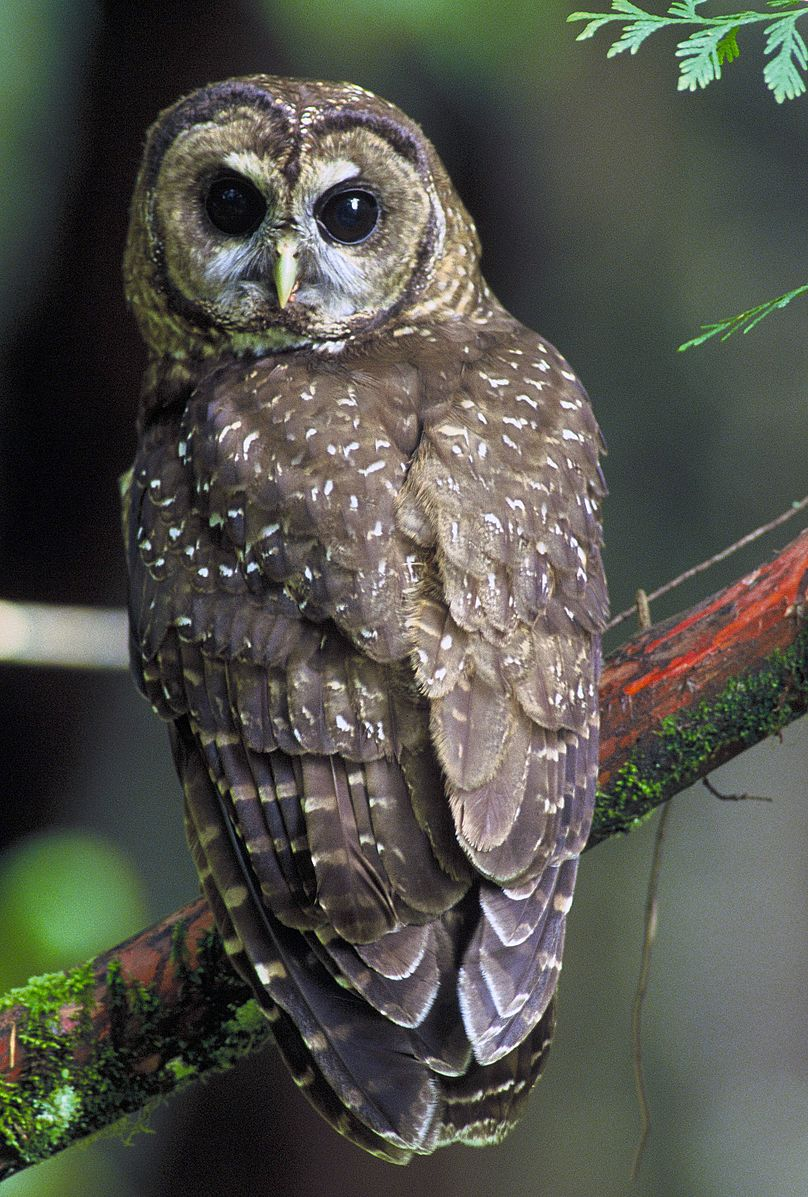
\includegraphics[width=.2\textwidth]{../images/NorthernSpottedOwl_USFWS}
\end{figure}

For these reasons, the managing entity, the United States Forest Service (USFS), would like to perform fuel removals in the Drink in order to reduce the area's fire hazard. However, performing these fuel removals has the potential to disrupt the habitat of the NSO \cite{bond2002short} and to induce short-term increases in sediment delivery \cite{o2005conceptual}. The latter is expected to be especially true in the Drink Area, where local USFS staff have noted that the watershed is unusually susceptible to spikes in sediment delivery as a result of foot traffic and other activities that occur within the watershed.

We developed a multi-objective mathematical program that optimizes the joint provision of these conflicting ecosystem services\footnote{These represent only a subset of the ecosystem services of concern to the USFS in the Drink Area. While the USFS manages for many ecosystem services simultaneously, many of the services are stacked rather than bundled, meaning the ecosystem services are not in conflict. These services need not all be considered in the multi-objective model, because the selection and maximization of one ecosystem service entails the maximization of all in the stack. For this reason, we have disregarded non-conflicting ecosystem services and selected a minimal bundle on which to employ multi-objective optimization. Those that do not conflict can be stacked post-optimization.}.

\section{The multi-objective model}
The multi-objective model is a zero-one mathematical program that assigns spatiotemporal prescriptions for fuel removals across the Drink Area to optimize the joint provision of ecosystem services. Spatially, the model prescribes fuel removals across 303 forest treatment units into which the Drink has been divided (the interior polygons in Figure \ref{fig:drinkOverview}). Temporally, the model operates over an 80-year planning horizon, from 2015 to 2095. The fuel removals are scheduled in two 20-year treatment periods: 2015-2035 and 2035-2055. For each treatment unit, the model may prescribe fuel removals in the first period, the second period, neither, or both.

To ensure long-term efficacy of the fuel removals, the model minimizes the fire hazard rating of the Drink Area at the end of the 80-year planning horizon. To mitigate impacts of the fuel removals on NSO habitat, the model maximizes the area of NSO habitat at the end of each planning period. Similarly, the model minimizes the short-term spikes in sediment delivery resulting from the application of fuel removals, which are assumed to be performed at the midpoint year in the treatment periods (years 2025 and 2045). Note that because a wildfire would is is expected to severely degrade NSO habitat and cause a mass delivery of sediment, we assume that the long-term minimization of fire hazard serves as a proxy for both the long-term protection against a mass sediment delivery event and for the protection of habitat for the northern spotted owl.

Figure \ref{fig:drinkPlanningHorizon} contains a schematic of the planning horizon which shows the timing of these events.

\begin{figure}
\centering
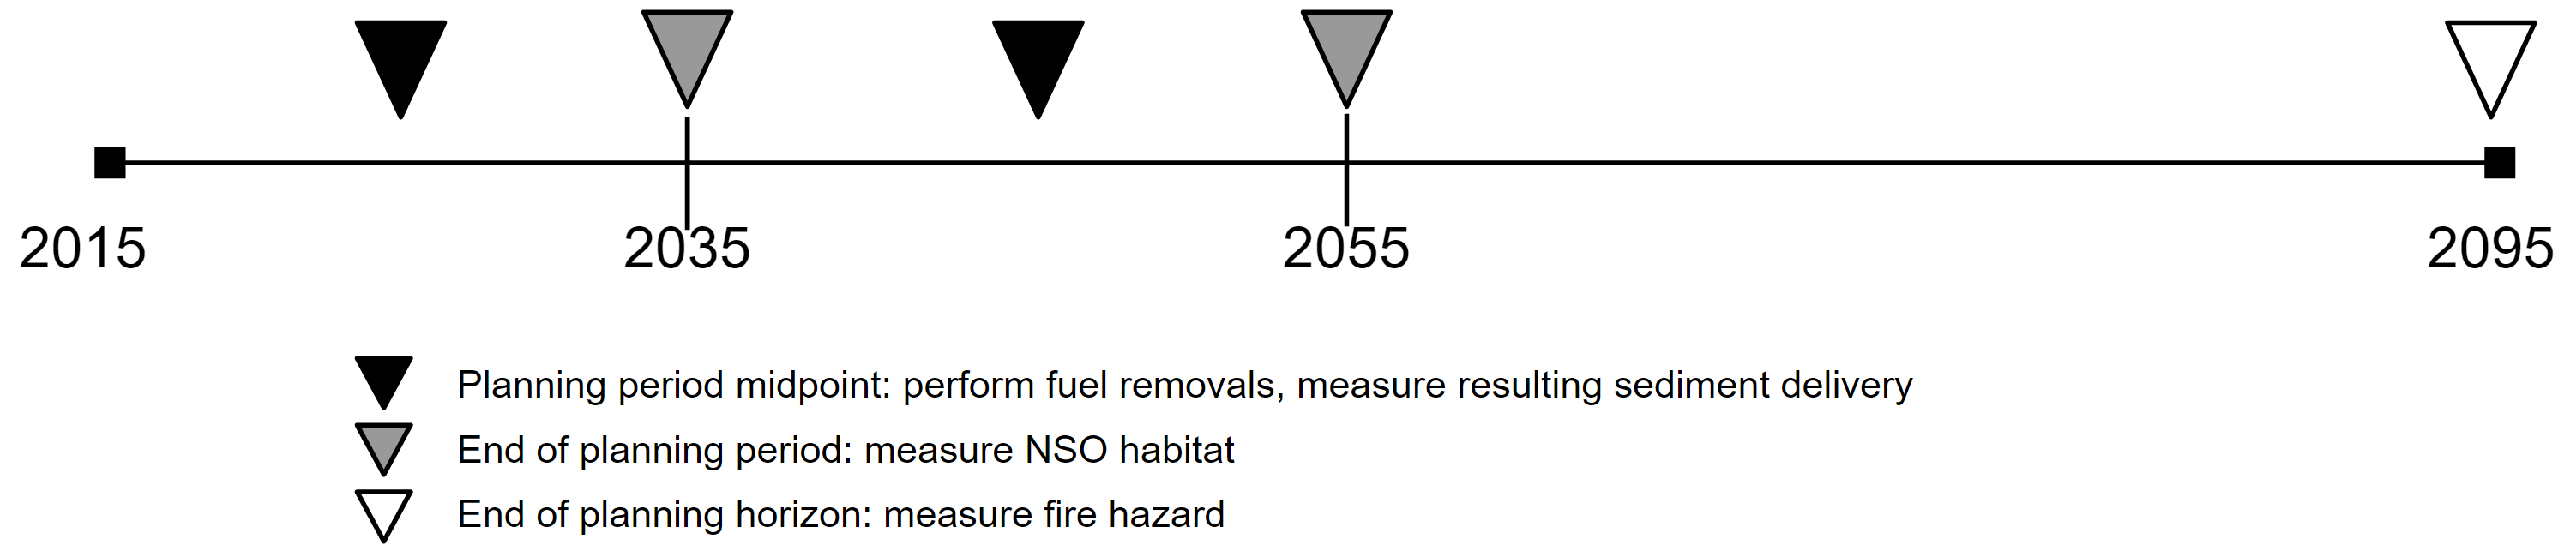
\includegraphics[width=.9\textwidth]{../images/Drink_PlanningHorizon_Sketch}
\caption[Planning horizon for the case study]{The planning horizon used in the case study spans the 80 year period from 2015 to 2095. Fuel removals may be performed in the first period (2015-2035), the second period (2035-2055), both, or neither. Fuel removals are assumed to be performed at the mid-point years of each period (black triangles). Sediment delivery is measured on treatment years. Treatment units' suitability for NSO habitat is measured at the end of the planning periods (gray triangles), and treatment units' fire hazard ratings are measured at the end of the planning horizon (white triangle).}
\label{fig:drinkPlanningHorizon}
\end{figure}

\subsection{Notation}
\label{subsec:notation}
We use the following notation in the development of the model:

\paragraph{Model parameters}
\begin{itemize}
\item \textbf{$i \in I$:} the set of treatment units comprising the Drink Area ($|I| = 303$)

\item \textbf{$a_i$:} the area of treatment unit $i$

\item \textbf{$r \in R$:} the set of fuel removal prescriptions:
	$$
	r =
	\begin{cases}
	1 &\text{ fuel removals in the first period (2015-2035)}\\
	2 &\text{ fuel removals in the second period (2035-2055)}\\
	3 &\text{ fuel removals in both periods}\\
	0 &\text{ no fuel removals performed in either period}
	\end{cases}
	$$
	
\item \textbf{$F_{i,r}$:} the area-weighted fire hazard rating of treatment unit $i$ at the end of the planning horizon if prescribed to fuel removal schedule $r$. For instance, if a treatment unit $i$ under fuel removal schedule $r$ has a fire hazard rating of 4 in the year 2095, and its area is 10 hectares, then $F_{i,r} = 40$. The metric for fire hazard rating used in this analysis was developed by Schroder \textit{et al.} \cite{schroder2016multi} specifically for the Drink Area. It uses fire characteristics from the set of fuel models proposed by Anderson \cite{anderson1982aids} in order to assign a fire hazard rating. We expand the rating system to include fuel models not present in Schroder \textit{et al.} See Table \ref{tab:firehazards} for the mapping of fuel models to fire hazard ratings.

The USFS's Climate-Forest Vegetation Simulator (Climate-FVS) was used to generate the fuels and vegetation characteristics of the treatment units in order to determine their fire hazard rating. Initial vegetation data for Climate-FVS came from the 2012 GNN structure map (\url{http://lemma.forestry.oregonstate.edu/data/structure-maps}) from Oregon State University's Landscape Ecology, Modeling, Mapping \& Analysis (LEMMA) group. Plots from the LEMMA database were mapped to the treatment units in the Drink area in order to produce tree and treatment unit lists. These lists were used with Climate-FVS to simulate the treatment units' vegetation and fuels characteristics forward for the duration of the planning horizon under each climate scenario. Input climate data for Climate-FVS was obtained through the Climate-FVS climate data server \cite{climateFVSReadyData}.

\begin{table}[!ht]
\centering
\resizebox{\textwidth}{!}{%
\begin{tabular}{lccrrr}
\multicolumn{1}{c}{Fuel Model} & \multicolumn{1}{c}{\textbf{Fire Hazard Rating}} & \multicolumn{1}{c}{Group} & \multicolumn{1}{c}{Flame length (m)} & \multicolumn{1}{c}{Rate of spread (m/hr)} & \multicolumn{1}{c}{Total fuel load (tons/ha)} \\ \hline
4*                              & \textbf{5}                                       & Shrub                     & 5.79                                 & 1508.76                                   & 32.12                                         \\
5                               & \textbf{4}                                       & Shrub                     & 1.22                                 & 362.10                                    & 8.65                                          \\
8                               & \textbf{1}                                       & Timber                    & 0.30                                 & 32.19                                     & 12.36                                         \\
9*                              & \textbf{2}                                       & Timber                    & 0.79                                 & 150.88                                    & 8.65                                          \\
10                              & \textbf{2}                                       & Timber                    & 1.46                                 & 158.92                                    & 29.65                                         \\
11*                             & \textbf{2}                                       & Logging Slash             & 1.07                                 & 120.7                                     & 28.42                                         \\
12                              & \textbf{4}                                       & Logging Slash             & 2.44                                 & 261.52                                    & 85.50                                         \\
13                              & \textbf{5}                                       & Logging Slash             & 3.20                                 & 271.58                                    & 143.57                                       
\end{tabular}%
}
\caption[Fire hazard ratings used in multi-objective model]{Fire hazard rating system used here, originally employed by Schroder \textit{et al.} \cite{schroder2016multi}. Non-forested areas are assigned a fire hazard value of 0.\\
Asterisks (*) denote fuel models not present in Schroder \textit{et al.}\\
The fuel model column refers to the Anderson fuel model ratings \cite{anderson1982aids}.}
\label{tab:firehazards}
\end{table}

\item \textbf{$I_{\omega,t}$:} the set of treatment units that qualify as NSO habitat at the end of planning period $t$ under at least one fuel removal schedule. The treatment units that qualify as NSO habitat at the end of a planning period $t$ are those that meet the following three criteria in year $t$, as specified by the USFS:
	\begin{enumerate}
	\item elevation less than 1830 m
	\item the presence of trees with diameter at breast height (DBH) at least 76 cm
	\item canopy closure of at least 60\%
	\end{enumerate}
The elevation requirement was checked using a digital elevation model from the US Department of Agriculture's GeoSpatial Data Gateway; canopy closure and large tree criteria were determined using the simulated vegetation characteristics output from Climate-FVS.

In addition, to account for the large habitat requirements of the NSO, treatment units must be members of a cluster exceeding 200 ha in size, the entirety of which meets the aforementioned NSO habitat criteria. Treatment units that meet the first three criteria but are not part of such a cluster are less valuable NSO habitat and therefore have their contributions to the total owl habitat discounted by a factor of $e$.

\item \textbf{$e$:} the discount factor applied to NSO habitat when it is not part of a contiguous habitat cluster at least 200 ha in size. Following the convention used in Schroder \textit{et al.} \cite{schroder2016multi}, we set $e = 0.5$.

\item \textbf{$j \in R_{i,t}$:} the set of fuel removal schedules such that treatment unit $i$ qualifies as NSO habitat at the end of planning period $t$. For instance, consider treatment unit $i=15$ and planning period $t=2$ (2035-2055). We seek to find the set of fuel removal prescriptions $r \in R$ such that treatment unit 15 is suitable NSO habitat at the end of planning period 2 (in year 2055). We enumerate the vegetation characteristics of treatment unit 15 for all possible fuel removal schedules and determine that if fuel removals are assigned in the second planning period, then treatment unit 15 does not qualify as NSO habitat in year 2055. Thus, $R_{15,2} = \{0,1\}$, since for $r=0$ (no fuel removals performed) and $r=1$ (fuel removals performed in first period only), treatment unit 15 does qualify as NSO habitat in 2055.

\item \textbf{$s_{i,t}$:} the amount of sediment (in tonnes) delivered to the watershed as a result of performing fuel removals on treatment unit $i$ in planning period $t$. The contributions of sediment delivery from treatment of treatment unit $i$ in period $t$ were determined using the online GIS tool for the Watershed Erosion Prediction Project (WEPP) \cite{frankenberger2011development}. WEPP GIS was selected for use, because it is able to take climate variables into account. The climate variables used in our simulations are the same custom climate data described above for use with Climate-FVS, obtained through the Climate-FVS data server.

WEPP GIS also takes soil textures, treatment types, and duration of simulation as inputs. Soil texture data for the Drink area was obtained from the USDA's Soil Survey Geographic (SSURGO) database, treatment types are those specified in \S \ref{chap:appendix_drinkTreatments}, and the years of simulation correspond to the treatment years in the planning horizon (2015-2095).

\item \textbf{$c \in C$:} Recall that the quantification of NSO habitat depends on the availability of large contiguous habitat patches; areas of NSO habitat less than than 200 ha in size are discounted. In order to determine when habitat is provided in sufficiently large areas, we must enumerate the set of clusters of treatment units whose combined area exceeds 200 ha. This set of clusters is the set $C$.

\item \textbf{$i \in D_c$:} Given a cluster $c \in C$, the set $D_c$ is the set of treatment units that comprise cluster $c$.

\item \textbf{$c \in C_i$:} Given a treatment unit $i$, we define the set $C_i$ as the set of clusters that contain treatment unit $i$

\item \textbf{$A$:} the maximum area in hectares that may be treated in either planning period. We constrain the allowable treatment area per period to account for the limited availability of work crews to perform the fuel removals. Following guidance from the USFS, we set $A = 2428$ ha (approximately 6000 ac).

\item \textbf{$\ell$, $u$:} the lower and upper bounds, respectively, on the relative fluctuation in the area treated in periods 1 and 2. These bounds are used to enforce regulation in the workflow for the USFS. Here we use values such that the area for which fuel removals are performed does not fluctuate more than 20\% between treatment periods; that is, we set the lower bound $\ell = 0.8$ and the upper bound $u = 1.2$.
\end{itemize}

\paragraph{Decision Variables}
$$
x_{i,r} = \begin{cases}
1 &\text{ if treatment unit $i$ is prescribed to treatment schedule $r$}\\
0 &\text{ otherwise}
\end{cases}
$$ 

\paragraph{Indicator Variables}
\begin{itemize}
\item \textbf{$q_{c,t} = 1$} if all treatment units in cluster $c$ qualify as NSO habitat at the end of planning period $t$; $q_{c,t} = 0$ otherwise
\item \textbf{$p_{i,t} = 1$} if in planning period $t$ treatment unit $i$ is part of a cluster $c$ such that $q_{c,t} = 1$; $p_{i,t} = 0$ otherwise
\end{itemize}

\paragraph{Accounting Variables}
\begin{itemize}
\item \textbf{$S_t$:} the total sediment delivered to the watershed from performing fuel treatments in planning period $t$
\item \textbf{$O_t$:} the amount of NSO habitat (in hectares) at the end of planning period $t$
\item \textbf{$H_t$:} the total area (in hectares) treated in planning period $t$
\end{itemize}

\subsection{Model formulation}
The formulation of the multi-objective model is as follows:
\begin{align}
Minimize \quad & \notag\\
&\sum_{i\in I}\sum_{r\in R} F_{i,r} x_{i,r} \label{eqn:objFire} \\
&\max \{S_1,S_2\} \label{eqn:objSediment} \\
Maximize \quad & \notag\\
&\min \{O_1,O_2\} \label{eqn:objOwl}
\end{align}
Subject to:
\begin{align}
\sum_{i\in I_{\omega,t}} \left(a_i p_{i,t} + e a_i \left( \sum_{j \in R_{i,t}} x_{i,j}-p_{i,t} \right) \right) &= O_t \qquad \forall t \in \{1,2\} \label{eqn:constraintDefOwl}\\
\sum_{i\in I} \sum_{r\in 1,3} s_{i,1} x_{i,r} &= S_1 \label{eqn:constraintSediment1} \\
\sum_{i\in I} \sum_{r\in 2,3} s_{i,2} x_{i,r} &= S_2 \label{eqn:constraintSediment2} \\
\sum_{i \in D_c} \sum_{j \in R_{i,t}} x_{i,j} - |c| q_{c,t} &\ge 0 \qquad \forall t \in \{1,2\}, c \in C \label{eqn:constraintClusterTriggers} \\
\sum_{c \in C_i} q_{c,t} - p_{i,t} &\ge 0 \qquad \forall t \in \{1,2\}, i \in I_{\omega,t} \label{eqn:constraintPVarTriggers} \\
\sum_{r \in R} x_{i,r} &= 1  \qquad \forall i \in I \label{eqn:constraintOnePrescrip} \\
\sum_{i \in I} \sum_{r \in 1,3} a_i x_{i,r} &= H_1 \label{eqn:constraintAreaAcctg1} \\
\sum_{i \in I} \sum_{r \in 2,3} a_i x_{i,r} &= H_2 \label{eqn:constraintAreaAcctg2} \\
H_t &\le A \qquad \forall t \in \{1,2\} \label{eqn:constraintAreaRestr} \\
\ell H_1 - H_2 &\le 0 \label{eqn:constraintAreaFlucL} \\
-u H_1 + H_2 &\le 0 \label{eqn:constraintAreaFlucU} \\
x_{i,r}, p_i, q_c \in \{0,1\} \quad &\forall i \in I, r \in R, c \in C \label{eqn:constraintNonNeg}
\end{align}

Equations \eqref{eqn:objFire}-\eqref{eqn:objOwl} are the objective functions: equation \eqref{eqn:objFire} minimizes the cumulative fire hazard rating of the Drink Area at the end of the 80-year planning horizon, equation \eqref{eqn:objSediment} minimizes the maximum peak in sediment delivery for the two planning periods, and equation \eqref{eqn:objOwl} maximizes the minimum NSO habitat available at the end of the planning periods. Equation set \eqref{eqn:constraintDefOwl} defines the amount of NSO habitat available at the end of the planning horizons. Note that if treatment unit $i$ does not belong to a cluster of NSO habitat exceeding 200 hectares, then its area contribution to total NSO habitat is discounted by a factor of $e$. Equations \eqref{eqn:constraintSediment1} and \eqref{eqn:constraintSediment2} define the sediment delivered in planning periods one and two, respectively.

Inequality set \eqref{eqn:constraintClusterTriggers} controls the value of the cluster variables $q_{c,t}$ indicating clusters that meet the NSO habitat criteria in each of the planning periods. Inequality set \eqref{eqn:constraintPVarTriggers} controls the value of the $p_{i,t}$ variables indicating whether treatment unit $i$ is included in a cluster of NSO habitat at time $t$.

The set of equalities \eqref{eqn:constraintOnePrescrip} enforces the logical constraint that each treatment unit must be prescribed to exactly one fuel removal schedule. Equations \eqref{eqn:constraintAreaAcctg1} and \eqref{eqn:constraintAreaAcctg2} are accounting constraints for the total area treated in each planning period, and inequalities \eqref{eqn:constraintAreaRestr} ensure that this area does not exceed the predefined maximum. Inequalities \eqref{eqn:constraintAreaFlucL} and \eqref{eqn:constraintAreaFlucU} bound the fluctuation in treated area between the planning periods. Finally, constraint \eqref{eqn:constraintNonNeg} defines the decision and indicator variables as binary.

\section{Solution method}
We developed an implementation of T\'{o}th's Alpha-Delta algorithm \cite{TothThesis} to solve the model \eqref{eqn:objFire}-\eqref{eqn:constraintNonNeg} utilizing the IBM ILOG CPLEX optimization engine. For a problem with $M$ objectives, the Alpha-Delta algorithm finds the Pareto frontier by iteratively slicing the $M$-dimensional objective space with a tilted $M-1$-dimensional hyperplane. The algorithm was implemented using an alpha parameter of $\alpha = .01$ and delta parameters of $\delta_{Hab} = 1$ ha and $\delta_{Sed} = 2$ tonnes for the NSO habitat and sediment delivery objectives, respectively.

\section{Climate change scenarios}
\label{sec:climateChange}
Like other ecosystems, forests will undergo changes as a result of the changing climate. For instance, researchers anticipate new spatial distributions of tree species \cite{iverson1998predicting}, increased sediment delivery to streams \cite{Goode20121}, and increasing disturbance regimes such as wildfires, droughts, and insect infestations \cite{vose2012effects}. As these transformations occur, the ability of forests to provide ecosystem services will change.

The extent of change will likely depend on the severity of the realized climate change. Thus, to understand the potential impacts on ecosystem services, multiple climate change scenarios representing a range of severities should be considered. We use three in our case study: one scenario in which climate change is ignored, ``None''; one in which climate change is predicted to be mild, ``Ensemble RCP 4.5'' (also ``E45''); and one in which climate change is predicted to be severe, ``Ensemble RCP 8.5'' (also ``E85''). These scenarios differ in their assumption of the additional energy per unit area that will be absorbed by the atmosphere, a value known as radiative forcing (RF). E45 assumes an RF of 4.5 $W/m^2$ and E85 assumes 8.5 $W/m^2$. In general, larger values of RF correspond to more severe climate change.

A given value of radiative forcing does not map to a single prediction of climate change, because researchers may disagree in how the climate will respond to that amount of RF. This is why for a given RF numerous climate models exist. A common approach to handling the disagreement among the climate models is to use an ensemble of climate models that all assume the same RF. We adopt this approach here for our E45 and E85 scenarios.

Each of these scenarios corresponds to an ensemble of 17 climate models. These climate models originate from the Fifth Assessment (AR5) on climate performed by the Intergovernmental Panel on Climate Change (IPCC). The selection and assembly of the 17 climate models used in these ensembles was conducted by Cookston (2016) and the Climate-FVS team \cite{ClimateModelsInFVSEnsemble}.

The other scenario, None, ignores any effects of climate change. While the number of studies incorporating climate change is increasing, this is still a common assumption in modern studies such as Schroder \textit{et al}. (2013) \cite{schroder2016multi}. Because it has served as the basis for many past studies of ecosystem services, the None climate scenario serves as a control against which we will compare the other two.

Each climate scenario corresponds to a different parameterization of the model, since the vegetation, fuels, and sediment delivery data depend on climate. Thus, changing the climate scenario has the potential to affect the amount and location of NSO habitat, the effects of fuel removals on NSO habitat, the fire hazard of the Drink Area, the efficacy of the fuel removals in reducing fire hazard, and the sediment delivered as a result of fuel removals. This drives changes to the relationships among the ecosystem services as well, which we investigate using the aforementioned conflict measures.


\section{Results}
We parameterized and solved the multi-objective model (equations \eqref{eqn:objFire}-\eqref{eqn:constraintNonNeg}) for each of the climate scenarios, generating three efficient frontiers: $Z_{\text{None}}$, $Z_{E45}$, and $Z_{E85}$ for the None, Ensemble RCP 4.5, and Ensemble RCP 8.5 scenarios, respectively.  $Z_{\text{None}}$ consists of 51 solutions, $Z_{\text{E45}}$ consists of 701 solutions, and $Z_{\text{E85}}$ consists of 1083. Figure \ref{fig:frontiersAll} shows the frontiers in their 3-dimensional objective spaces, Figure \ref{fig:consolidatedFrontiers} shows all frontiers in a single 3-dimensional view, and Figure \ref{fig:frontiersPCPlot} provides a single parallel coordinates plot with all frontiers. The summary details of their objective achievements are listed in Table \ref{tab:frontiersSummary}.

\begin{table}[]
\centering
\caption[Summary of objective achievement across climate scenarios]{Summary of the performance of the efficient frontiers for each climate change scenario.}
\label{tab:frontiersSummary}
\begin{tabular}{lllll}
\multicolumn{2}{l}{}                                                  & \textbf{None} & \textbf{E45} & \textbf{E85} \\ \hline
\multirow{3}{*}{\begin{tabular}[c]{@{}l@{}}\textbf{Fire hazard (cumulative}\\ \textbf{area-weighted fire hazard)}\end{tabular}}       & \multicolumn{1}{l}{min} & 21,321.21      & 23,219.82     & 23,268.02     \\
                                            & \multicolumn{1}{l}{avg} & 21,406.26      & 23,324.41     & 23,369.57     \\
                                            & \multicolumn{1}{l}{max} & 21,933.29      & 23,973.79     & 23,724.98     \\ \hline
\multirow{3}{*}{\textbf{NSO habitat (ha)}}       & \multicolumn{1}{l}{min} & 2,532.33       & 2,412.18      & 2,171.10      \\
                                            & \multicolumn{1}{l}{avg} & 2,536.31       & 2,447.92      & 2,421.99      \\
                                            & \multicolumn{1}{l}{max} & 2,540.05       & 2,477.18      & 2,481.01      \\ \hline
\multirow{3}{*}{\textbf{Sediment delivery (tonnes)}} & \multicolumn{1}{l}{min} & 0             & 0            & 0            \\
                                            & \multicolumn{1}{l}{avg} & 10.25         & 27.98        & 31.19        \\
                                            & \multicolumn{1}{l}{max} & 24.57         & 63.43        & 69.68        
\end{tabular}
\end{table}


\begin{figure}[ht!]
  \subfloat[None]{%
    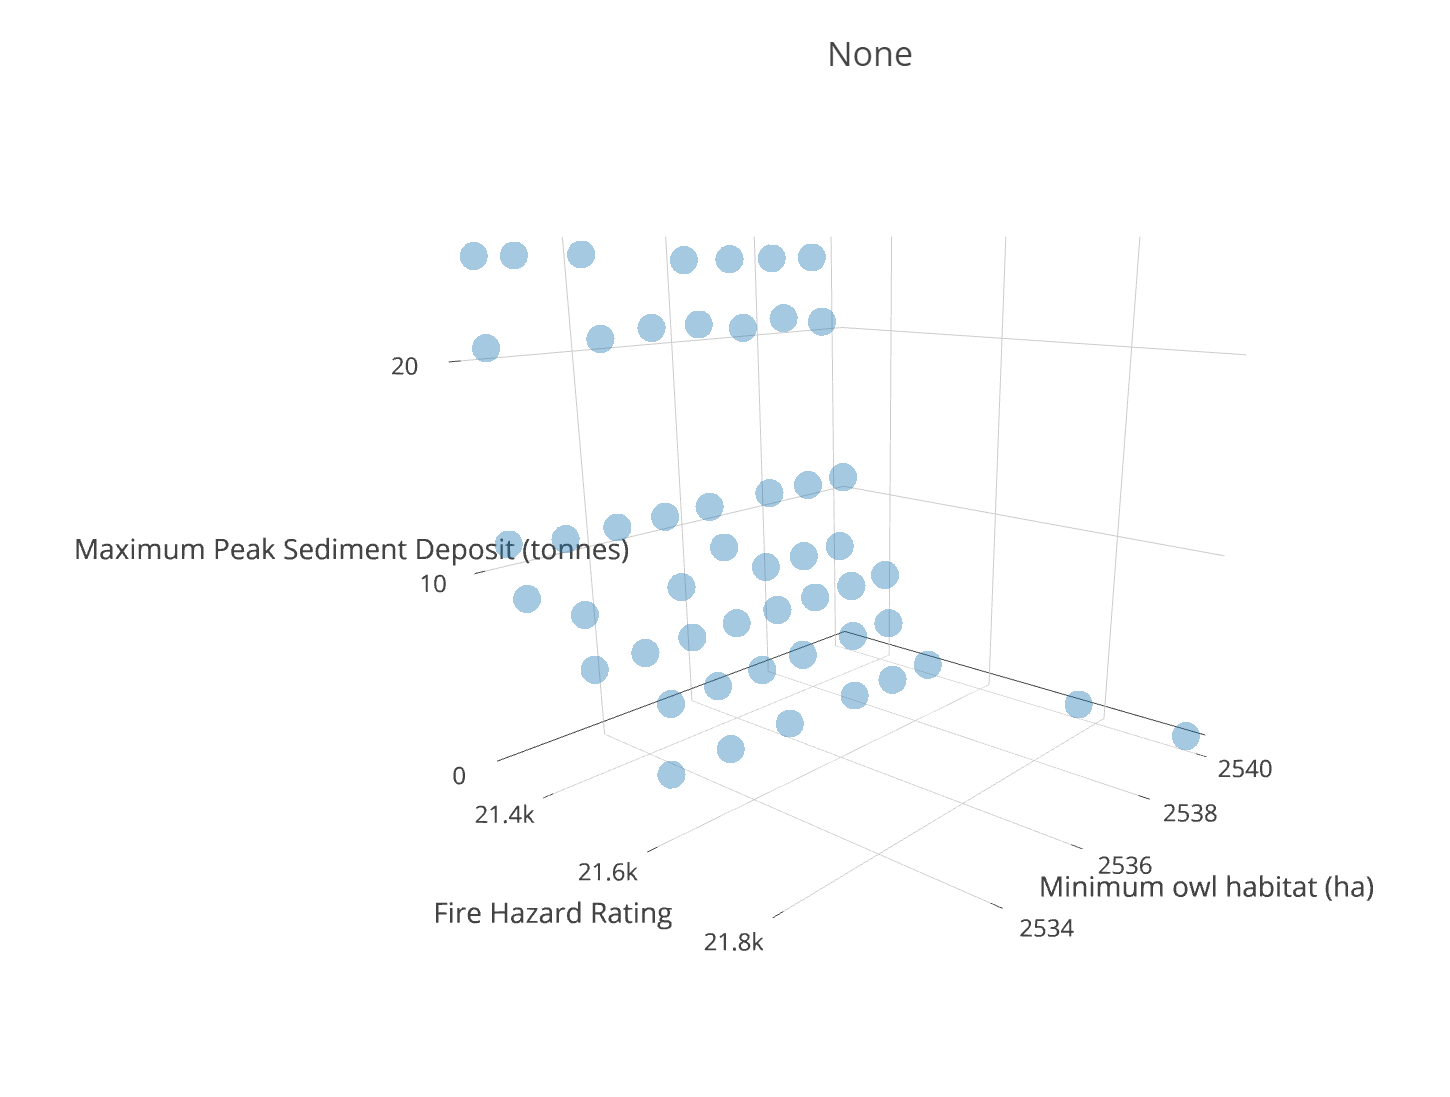
\includegraphics[width=.49\textwidth]{../images/Frontier_None}%
    \label{fig:frontierNone}%
  }
  \subfloat[Ensemble RCP 4.5]{%
    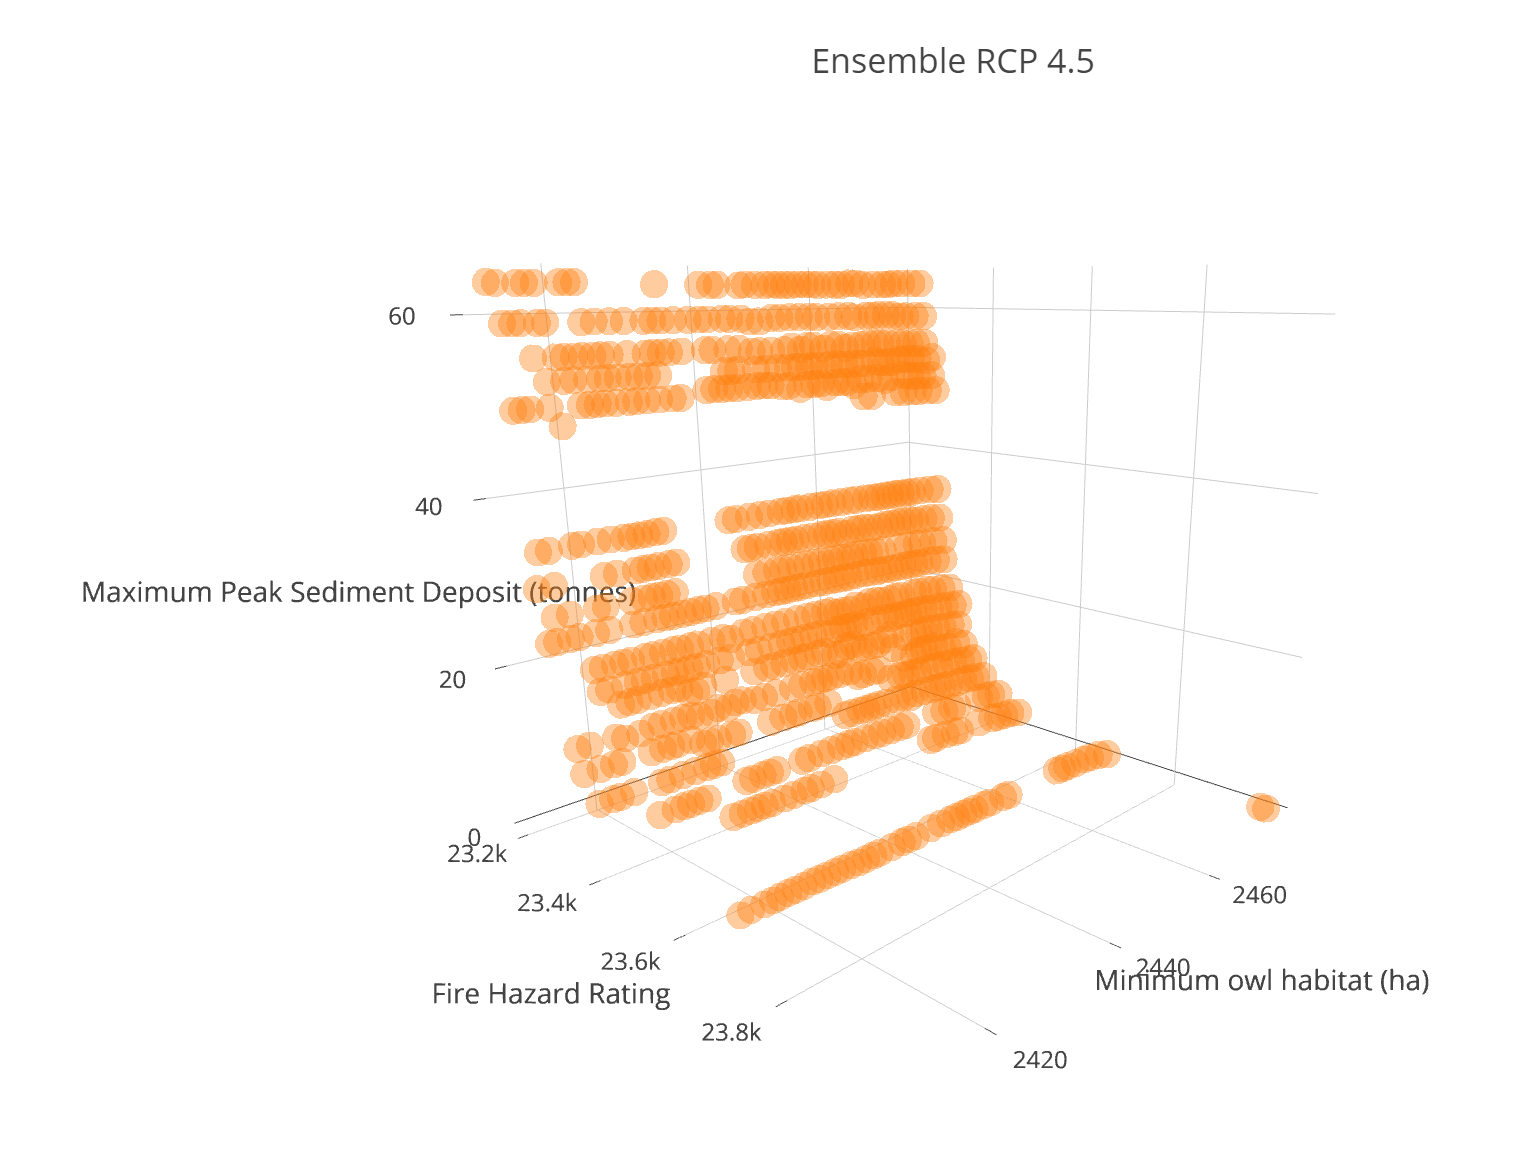
\includegraphics[width=.49\textwidth]{../images/Frontier_E45}%
    \label{fig:frontierE45}%
  }\hfill\centering
  \subfloat[Ensemble RCP 8.5]{%
    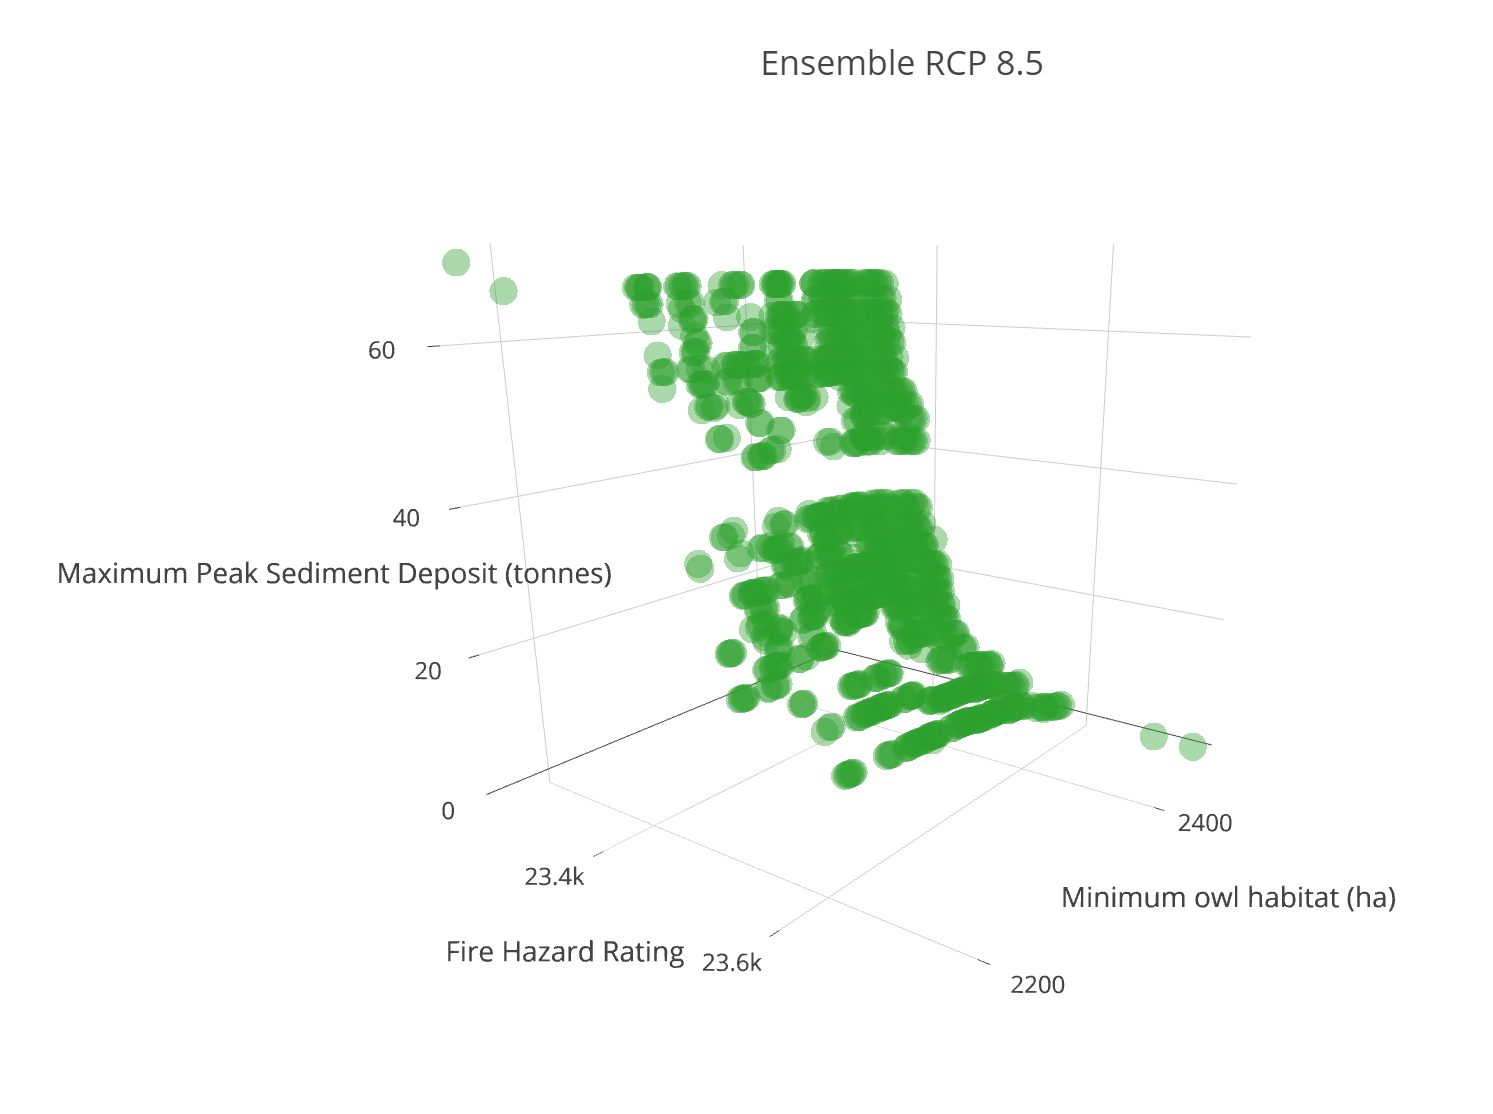
\includegraphics[width=.49\textwidth]{../images/Frontier_E85}%
    \label{fig:frontierE85}%
  }
  \caption[Frontiers for each climate change scenario]{Efficient frontiers for each climate change scenario.}
  \label{fig:frontiersAll}
\end{figure}

\begin{figure}[ht]
\centering
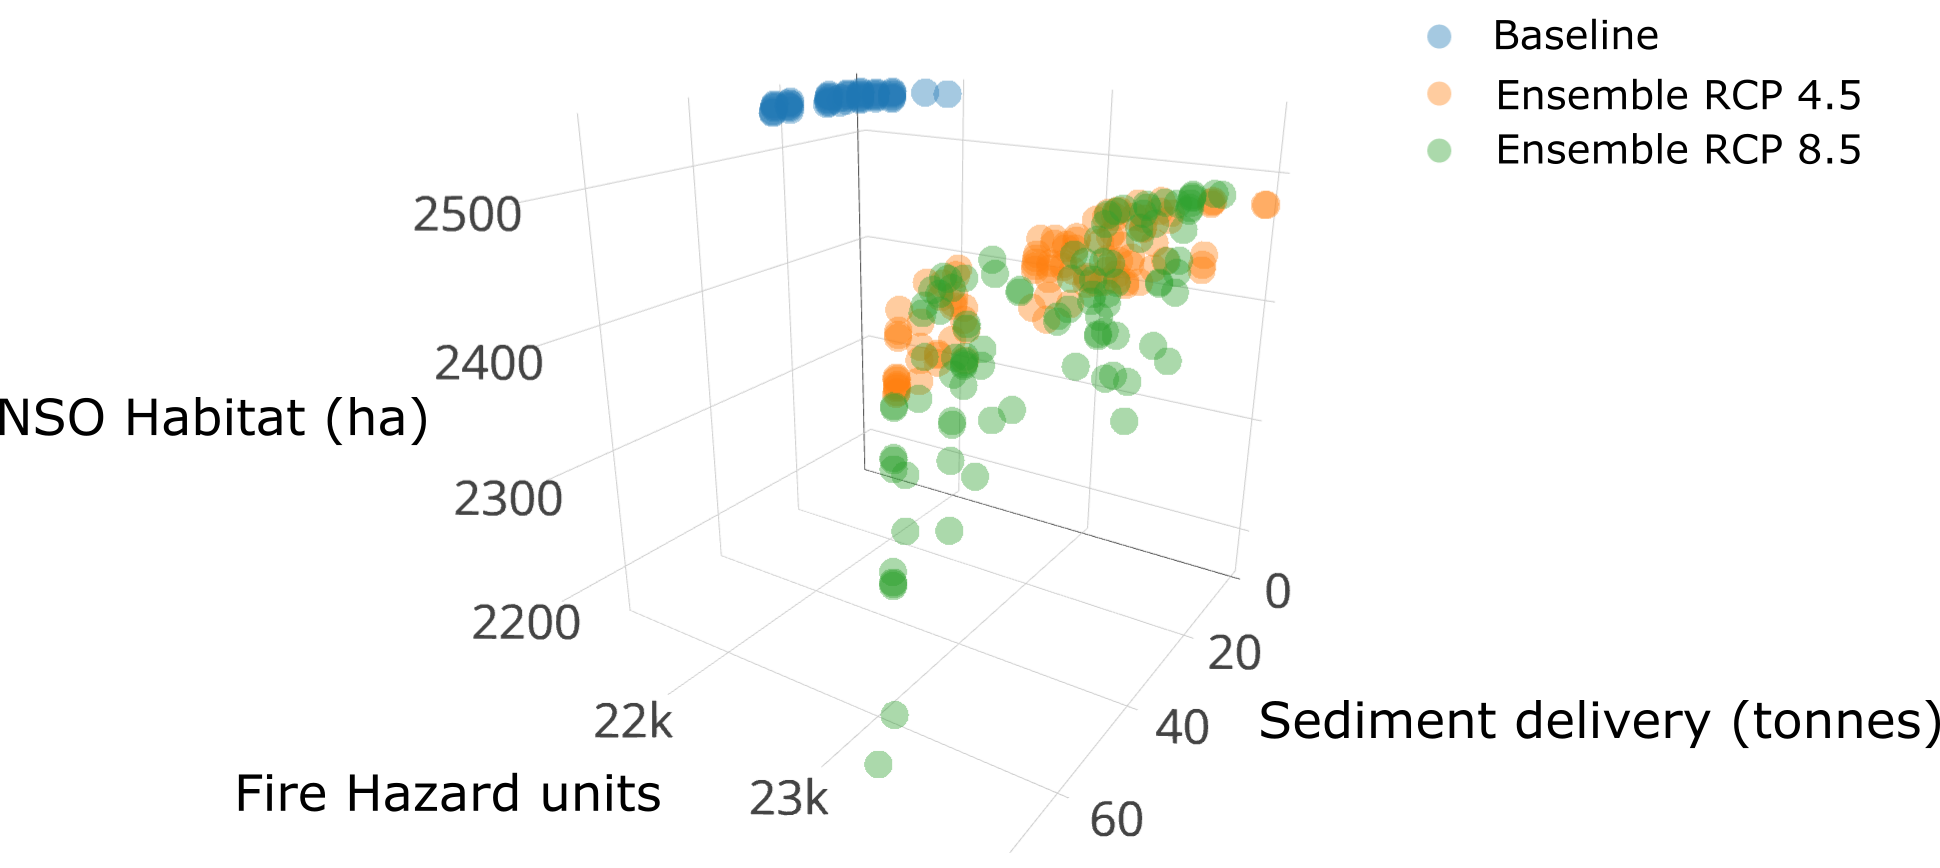
\includegraphics[width=.65\textwidth]{../images/consolidated3DFrontiers}
\caption[Unscaled 3D frontiers for all climate change scenarios]{Unscaled 3D frontiers for all climate change scenarios.}
\label{fig:consolidatedFrontiers}
\end{figure}

\begin{figure}[ht]
\centering
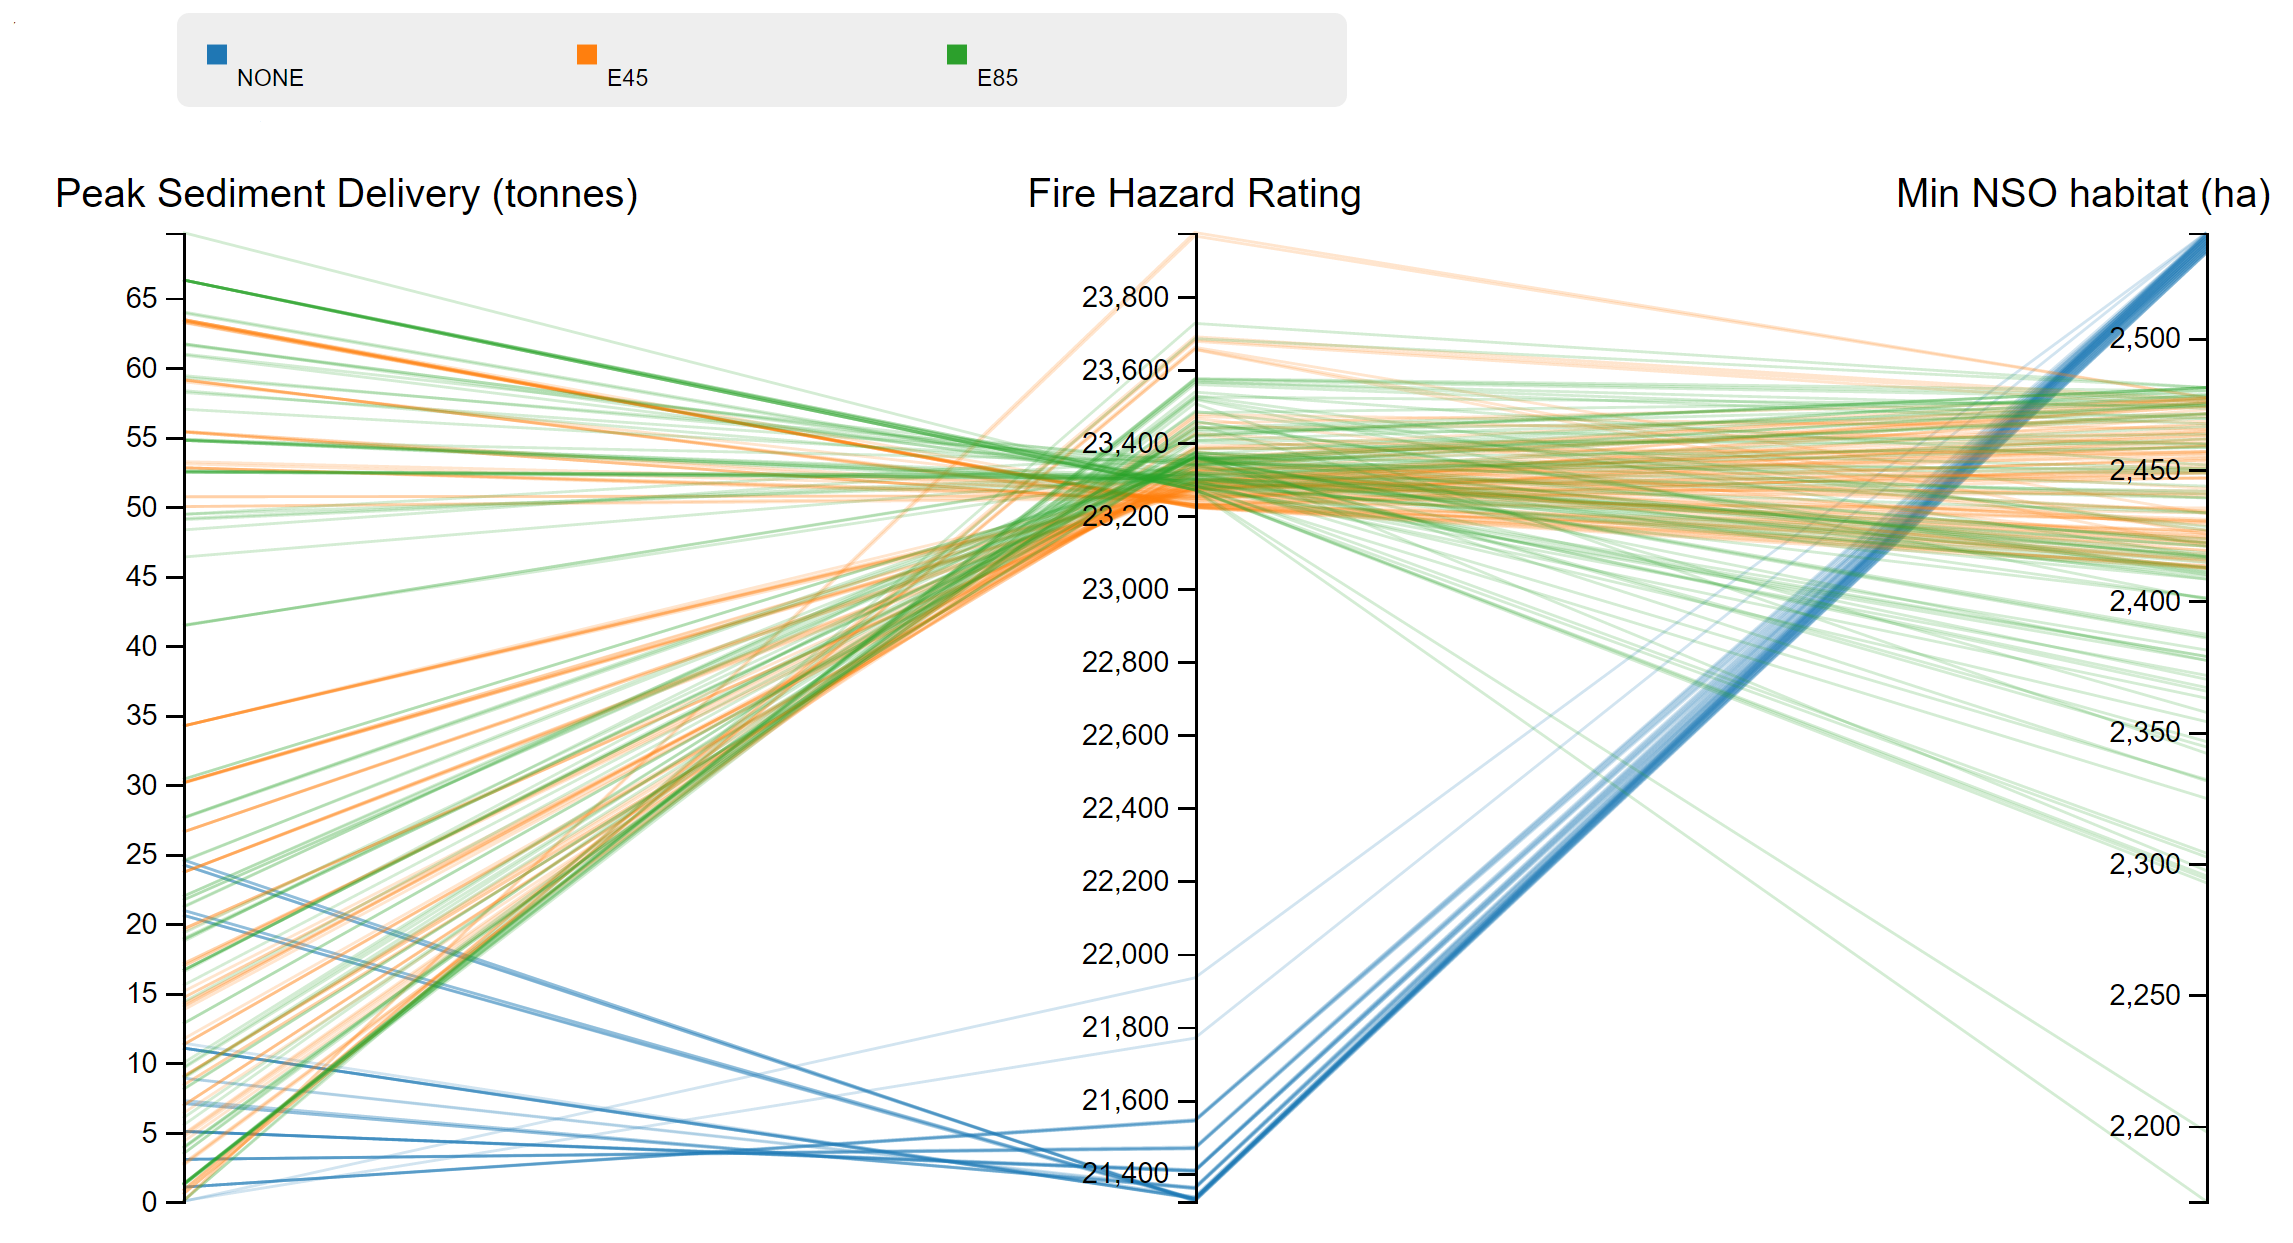
\includegraphics[width=.85\textwidth]{../images/FrontiersPCPlot}
\caption[Parallel coordinates view of the three frontiers]{Parallel coordinates view of the frontiers. Each axis represents an ecosystem service optimized by the model and each line represents a solution. In all objectives, we notice that None appears to outperform both the E45 and E85 scenarios, which show similar average objective achievements. To increase visual clarity, only a subset of solutions for E45 and E85 are shown.}
\label{fig:frontiersPCPlot}
\end{figure}

%We first report the impacts of climate change on the provision of individual ecosystem services before analyzing its impacts on the joint provision of ecosystem services and the conflict among them.

\subsection{Individual provision of ecosystem services}
The average achievement of all ecosystem services decreases with increasing severity of climate change -- see Table \ref{tab:frontiersSummary}. We find that the difference in ecosystem service provision is greater between the assumption of no climate change and mild climate change (None to E45) than it is between mild climate change and severe climate change (E45 to E85).

\paragraph{Sediment delivery} 
All scenarios have a lower bound on sediment delivery of 0, but the upper bound and the average sediment delivery both increase with climate change severity. Compared to the None scenario with an average sediment delivery of 10.25 tonnes, the average amount of sediment delivered in E45 is 27.98 tonnes, an increase of 172\%. The average for E85 is 31.19 tonnes, 204\% higher than None.

\paragraph{Fire hazard}
Similarly, we find that the average fire hazard of the Drink Area increases with climate change severity. The average for None is 21406.26 while E45 and E85 both perform approximately 9\% worse with an average of 23324.41 and 23369.57, respectively. This increase of 9\% in fire hazard is equivalent to the situation in which more than 1900 ha of the Drink area saw its fuel model raise from 5 to 13.

\paragraph{NSO habitat}
Finally, we also observe a decrease in the average provision of NSO habitat with increasing climate change. Compared to None which has an average provision of 2536.31 ha of NSO habitat, the average provision in the E45 scenario is 88.4 ha less (-3.5\%), and E85 is 114.3 ha less (-4.5\%).

We also find that for the sediment delivery and NSO habitat objectives, the range of achievable values increases with climate change severity. For sediment delivery, the range increases from 24.57 tonnes in None to 63.43 in E45 to 69.68 in E85. And for NSO habitat, the range increases from 7.72 ha in None to 65 ha in E45 and to 309.91 ha in E85.

\subsection{Conflict and the joint provision of ecosystem services}
As we saw for provision of individual ecosystem services, our results show that climate change will have an impact on conflict and the joint provision of ecosystem services as well.

We observe a decreasing hypervolume indicator with increasing severity of climate change -- see Table \ref{tab:hypervols}. The hypervolume for E45 is $0.0101$ less than None, and E85 is $0.0474$ less than None. However, all hypervolumes indicate frontiers which fill a large percentage of the objective space, as the smallest value (E85) is $I_{H1}(Z_\text{E85}) = 0.8295$. The binary hypervolumes (see Table \ref{tab:binaryHypervols}) tend to align with the hypervolumes, with larger values of $I_{H2}(Z_1,Z_2)$ when $I_{H1}(Z_1) > I_{H1}(Z_2)$ and smaller values when $I_{H1}(Z_2) > I_{H1}(Z_1)$. We note that no frontier is dominated by any other, as all binary hypervolume values in Table \ref{tab:binaryHypervols} are strictly positive.

\begin{table}[]
\centering
\caption[Hypervolumes of the efficient frontiers]{Hypervolume for each climate change scenario. Hypervolume values increase with increasing severity of climate change.}
\label{tab:hypervols}
\begin{tabular}{lllll}
\multicolumn{2}{l}{}                                                  & \textbf{None} & \textbf{E45} & \textbf{E85} \\ \hline
\multicolumn{2}{l}{\textbf{Hypervolume}}                              & 0.876977      & 0.866857     & 0.829541       
\end{tabular}
\end{table} 

\begin{table}[]
\centering
\caption[Binary hypervolume values for each pair of climate scenarios]{Binary hypervolumes for each pair of climate scenarios. No values are negative, indicating that no frontiers are dominated by another and that all frontiers uniquely enclose some volume of the objective space.}
\label{tab:binaryHypervols}
\begin{tabular}{lll}
\textbf{$Z_1$} & \textbf{$Z_2$} & \textbf{$I_{H2}(Z_1,Z_2)$} \\ \hline
\textbf{None}  & \textbf{E45}   & 0.026154                   \\
\textbf{None}  & \textbf{E85}   & 0.058001                   \\
\textbf{E45}   & \textbf{None}  & 0.016034                   \\
\textbf{E45}   & \textbf{E85}   & 0.045156                   \\
\textbf{E85}   & \textbf{None}  & 0.010565                   \\
\textbf{E85}   & \textbf{E45}   & 0.007841                  
\end{tabular}
\end{table}

\paragraph{Sediment delivery-NSO Habitat}
In the pairwise comparison of objectives, we observe little conflict between sediment delivery and NSO habitat under all climate scenarios. This is evident first in the proposed conflict metric $C_{ij}$, for which the largest value across all frontiers is 0.25 -- see Table \ref{tab:pairConflict-SedNSO}. We also notice the lack of conflict in Figure \ref{fig:pairplotNSOSed}. The figure shows the efficient frontier plotted in the sediment delivery-NSO habitat plane, where each objective has been normalized such that better values are higher and worse values are lower. For instance, in this graph, the point $(1,1)$ represents 0 sediment delivery and maximum NSO habitat. For all climate scenarios, we see similar uniform spreads of solutions as well as multiple solutions near the sub-dimensional ideal solution at $(1,1)$.

\begin{table}[]
\centering
\caption[Sediment-NSO conflict across climate scenarios]{Conflict between sediment delivery and NSO habitat across climate scenarios.}
\label{tab:pairConflict-SedNSO}
\begin{tabular}{llll}
\textbf{}     & \textbf{$C_{ij}$} & \textbf{$c_{ij,\rho}$} & \textbf{$c_{ij,d}$} \\ \hline
\textbf{None} & 0.19639           & 0.3974                 & 0.4942              \\
\textbf{E45}  & 0.25667           & 0.5194                 & 0.4941              \\
\textbf{E85}  & 0.19284           & 0.5160                 & 0.3737             
\end{tabular}
\end{table}


\begin{figure}[ht]
\centering
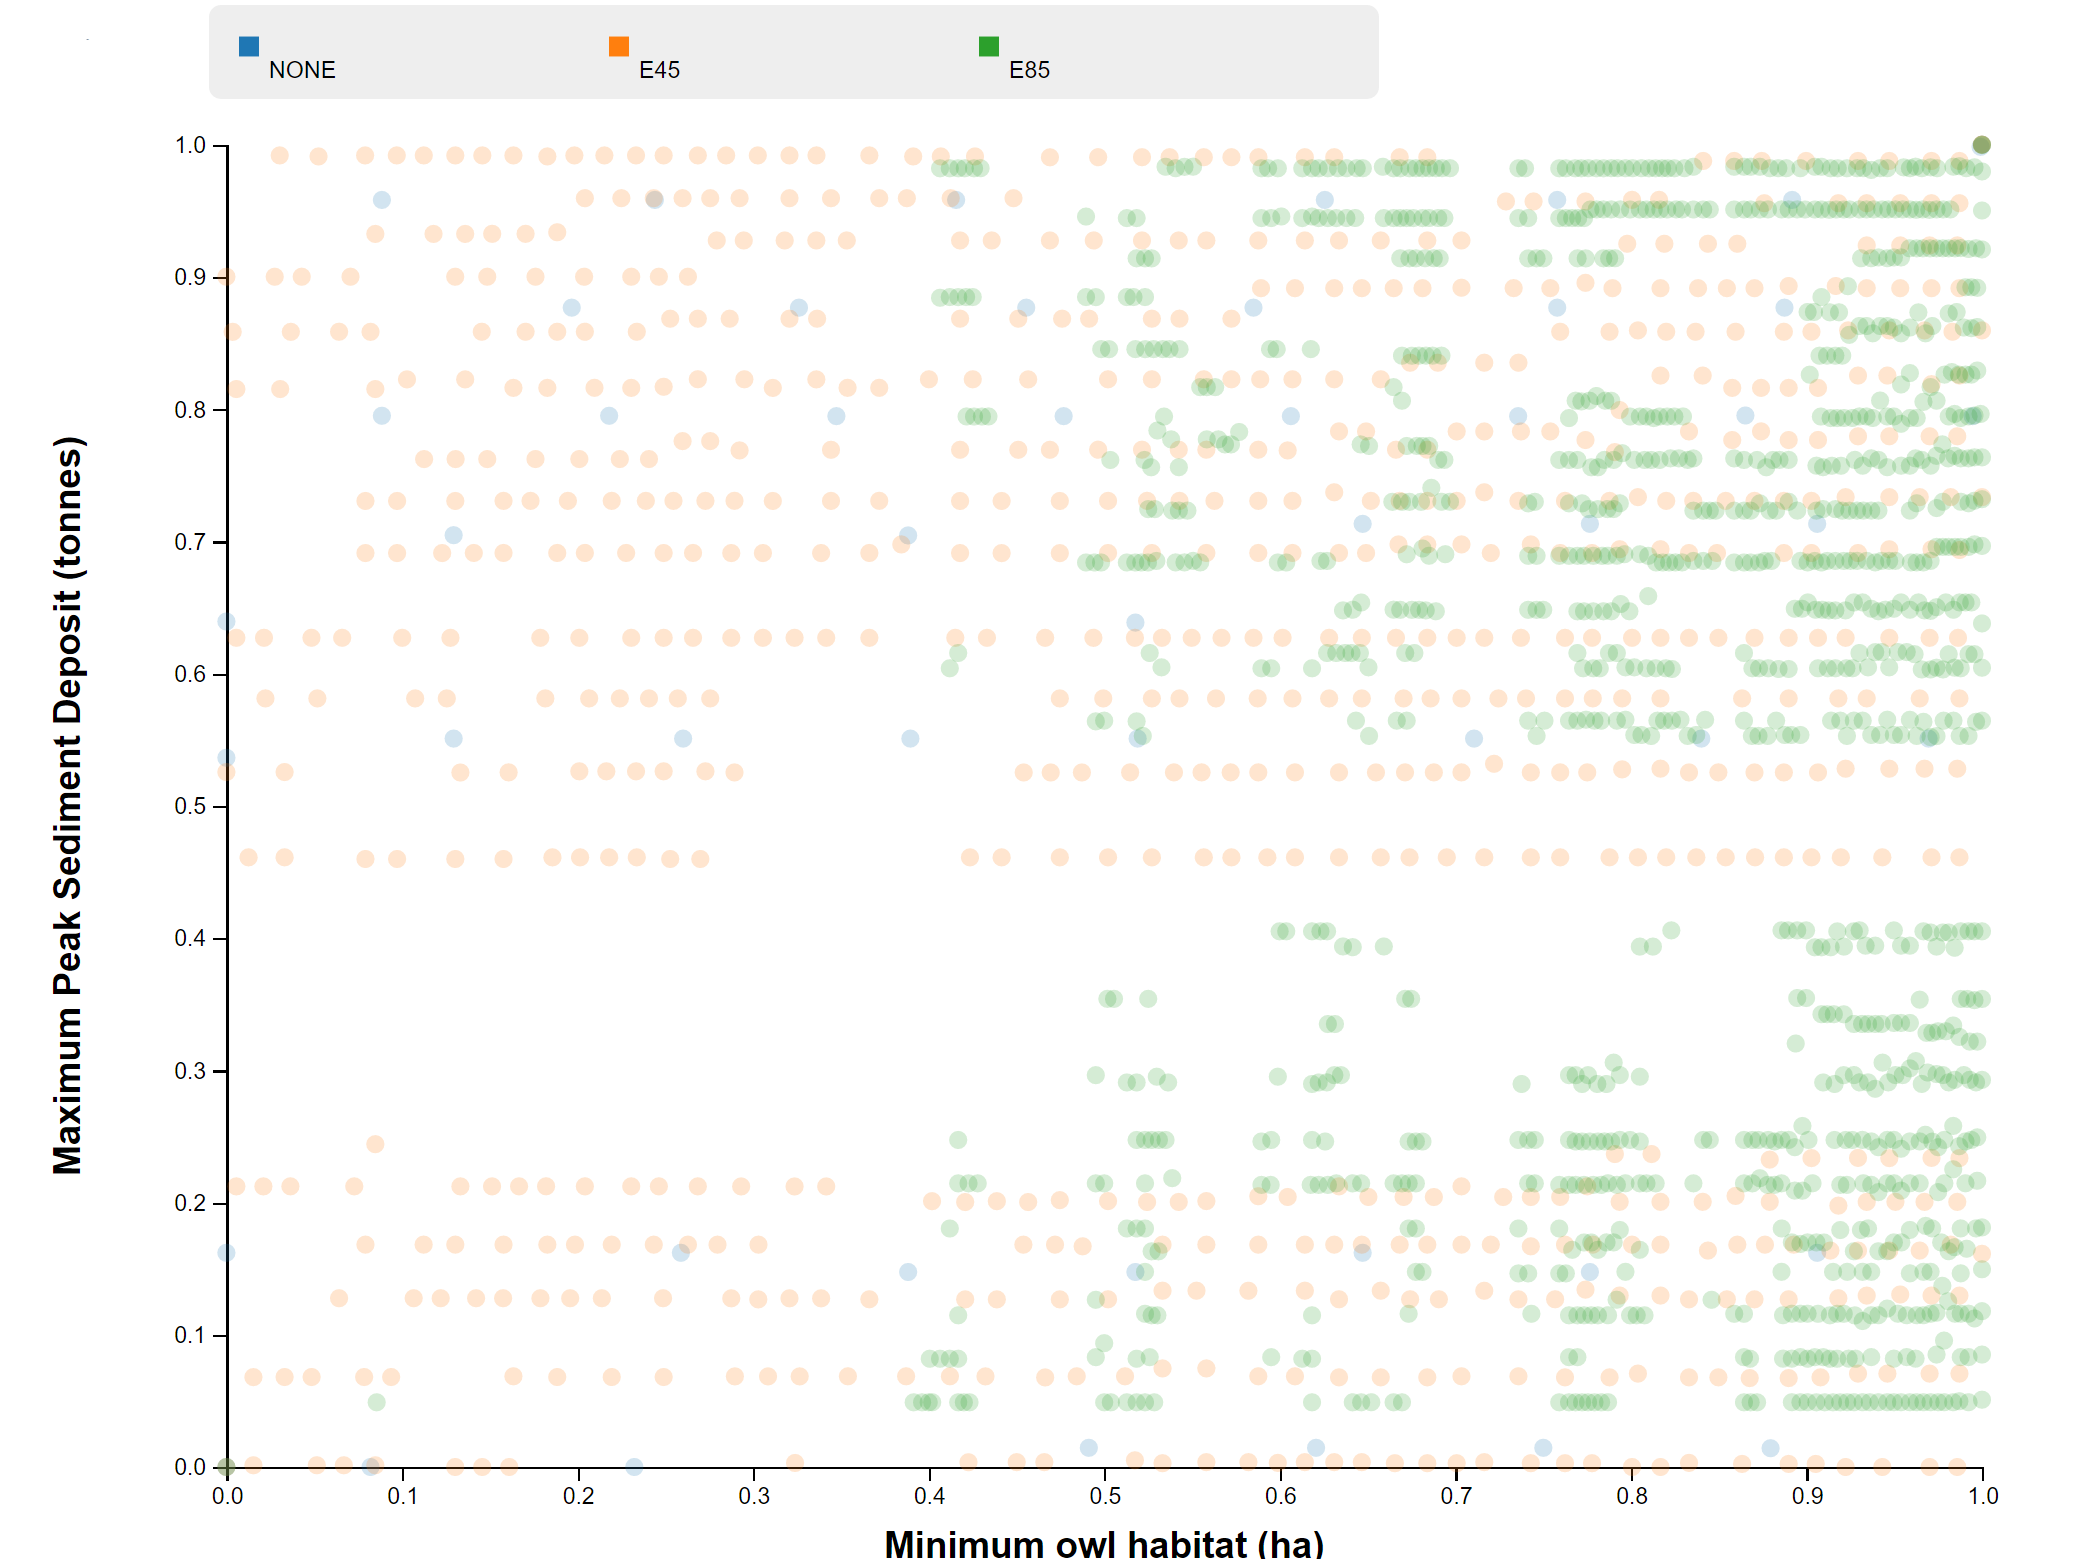
\includegraphics[width=.75\textwidth]{../images/2DSlice_NSO_Sed}
\caption[NSO habitat vs. sediment delivery for all climate scenarios]{NSO habitat versus sediment delivery for all climate scenarios. No obvious conflict pattern exists between the objectives in any climate scenario.}
\label{fig:pairplotNSOSed}
\end{figure}

\paragraph{NSO habitat-fire hazard}
According to $C_{ij}$, the conflict between NSO habitat and fire hazard is again small for all climate scenarios; however, it appears to decrease with increasing severity of climate change. We see in Table \ref{tab:pairConflict-NSOFire} that the average distance to the ideal decreases with increasing severity of climate change. See also Figure \ref{fig:pairplotNSOFire} which shows spreads of solutions for each climate scenario in the NSO habitat-fire hazard plane. The solutions are increasingly more clustered near the sub-dimensional ideal solution with increasing climate change severity.

\begin{figure}[ht]
\centering
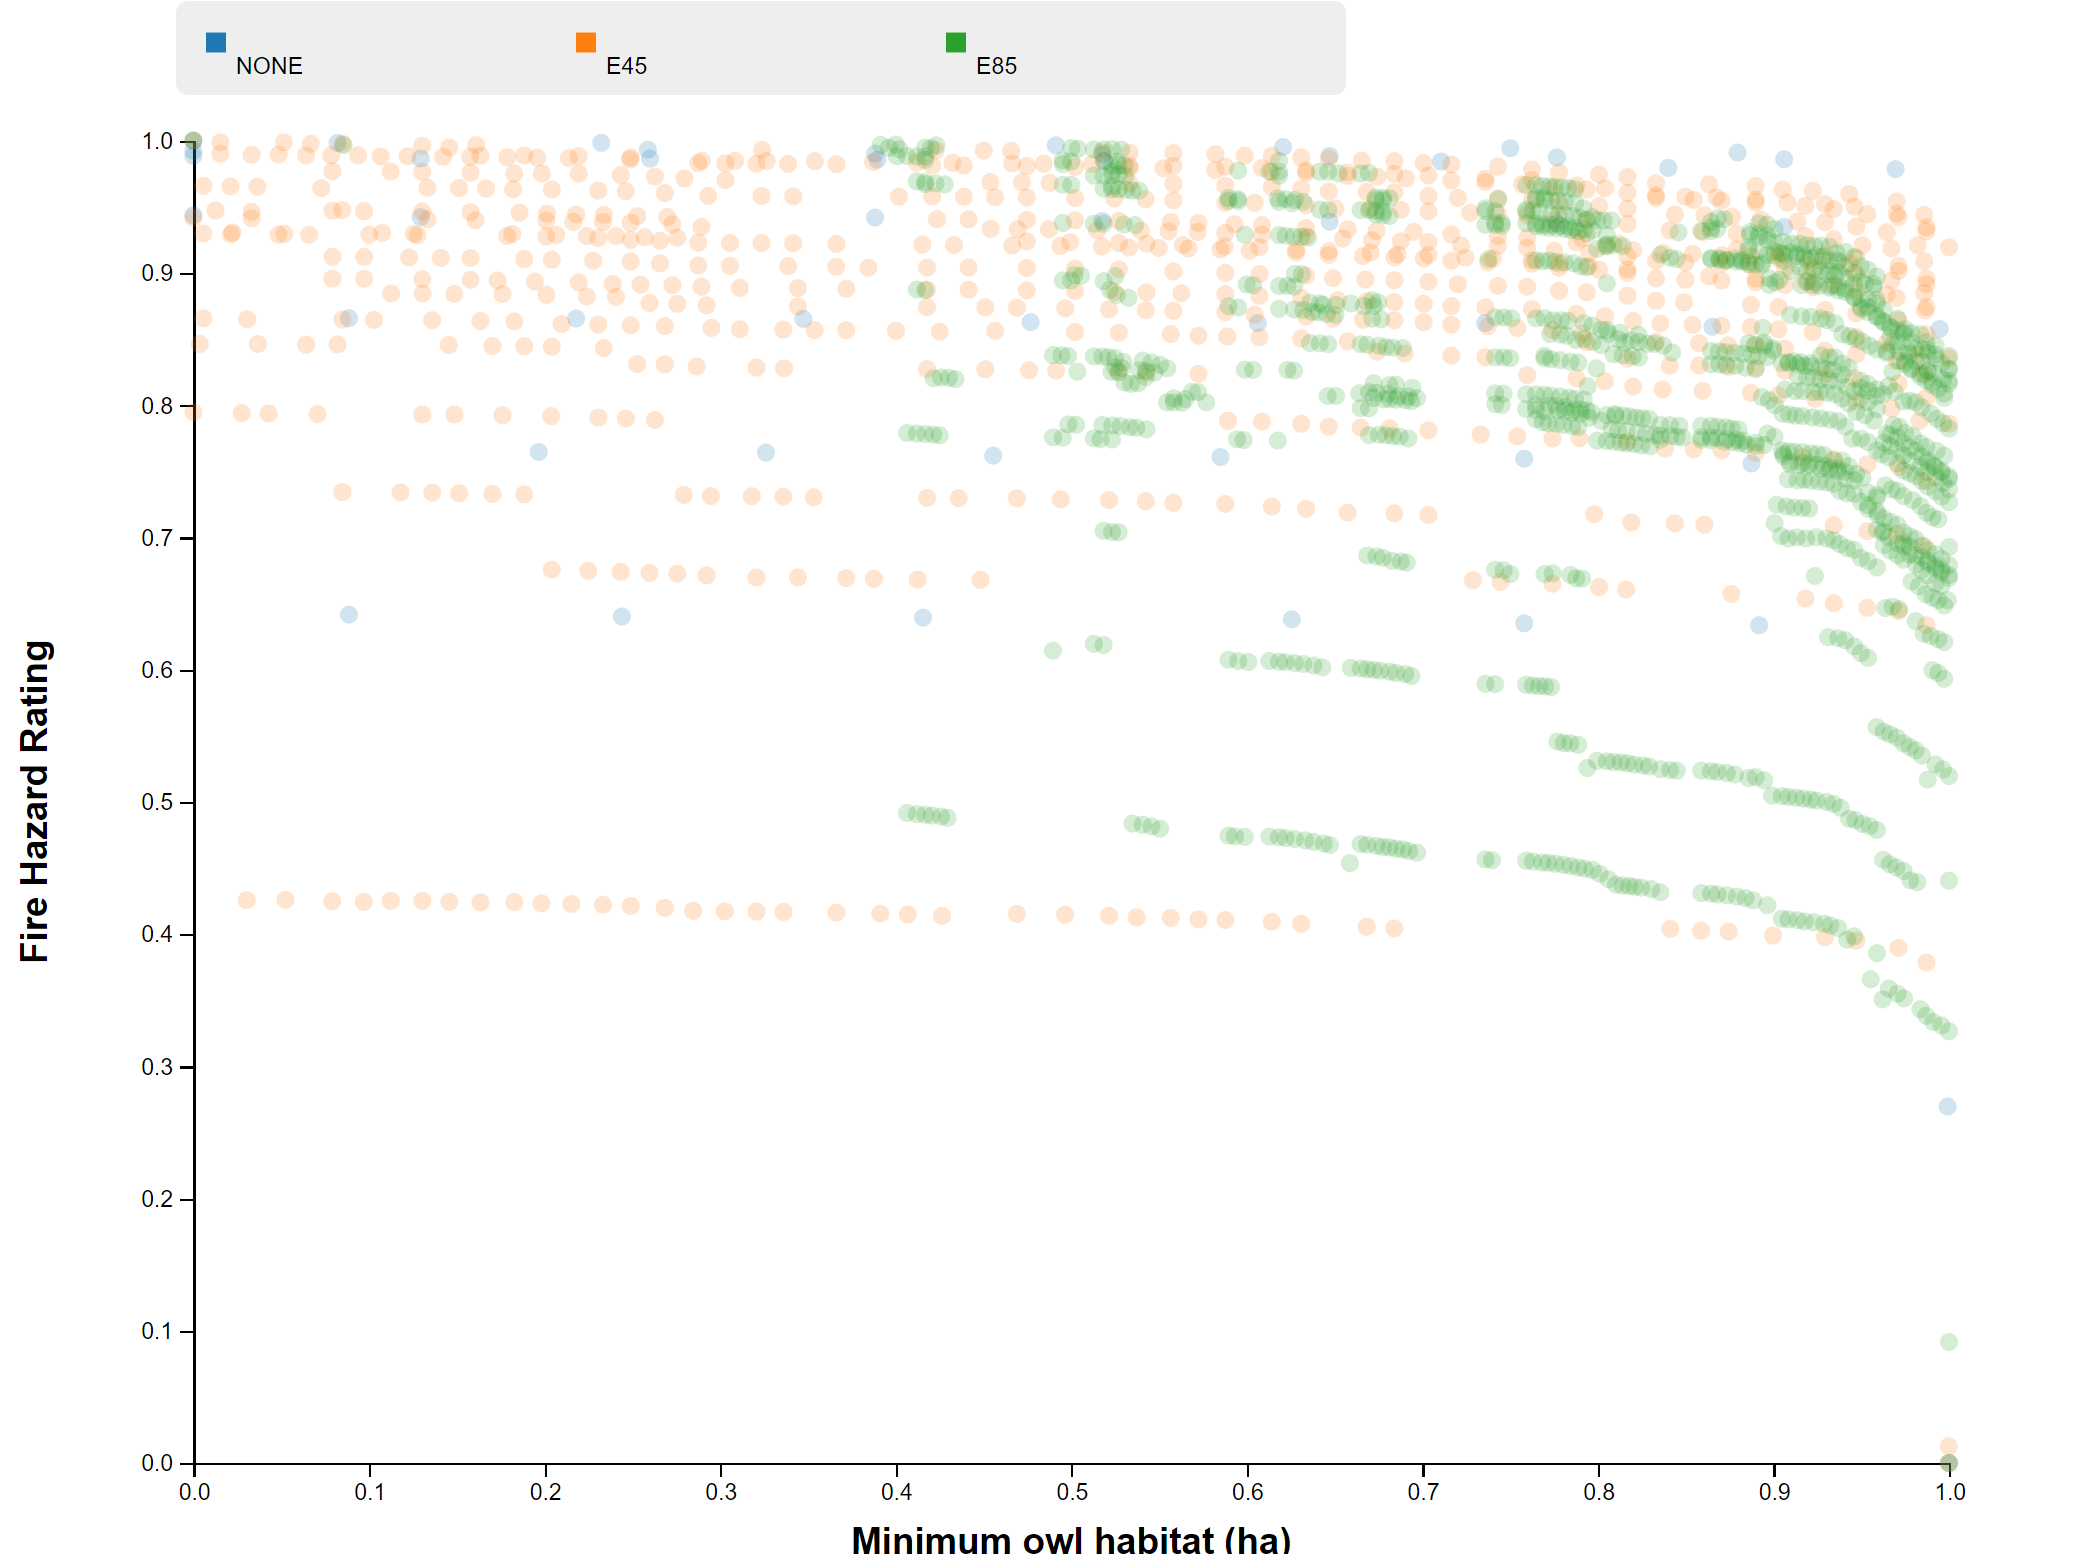
\includegraphics[width=.75\textwidth]{../images/2DSlice_NSO_Fire}
\caption[NSO habitat vs. fire hazard for all climate scenarios]{NSO habitat versus fire hazard for all climate scenarios.}
\label{fig:pairplotNSOFire}
\end{figure}

\begin{table}[]
\centering
\caption[NSO-fire hazard conflict across climate scenarios]{Conflict between NSO habitat and fire hazard across climate scenarios.}
\label{tab:pairConflict-NSOFire}
\begin{tabular}{llll}
\textbf{}     & \textbf{$C_{ij}$} & \textbf{$c_{ij,\rho}$} & \textbf{$c_{ij,d}$} \\ \hline
\textbf{None} & 0.25805           & 0.6622                 & 0.3897              \\
\textbf{E45}  & 0.20560           & 0.5807                 & 0.3541              \\
\textbf{E85}  & 0.15670           & 0.6643                 & 0.2359
\end{tabular}
\end{table}

\paragraph{Fire hazard-sediment delivery}
In all climate scenarios, the strongest pairwise conflict is between fire hazard and sediment delivery. This is apparent from both Figure \ref{fig:pairplotSedFire} and the conflict metric, Table \ref{tab:pairConflict-SedFire}. All rank correlation conflict values $c_{ij,\rho} > 0.95$, indicating strong negative rank correlation. In Figure \ref{fig:pairplotSedFire} we observe a clear void of solutions in all climate change scenarios near the sub-dimensional ideal solution at $(1,1)$; this is unlike Figures \ref{fig:pairplotNSOSed} and \ref{fig:pairplotNSOFire}. We also notice that the None and E45 solutions generally extend beyond the E85 solutions in this plane.

\begin{figure}[ht]
\centering
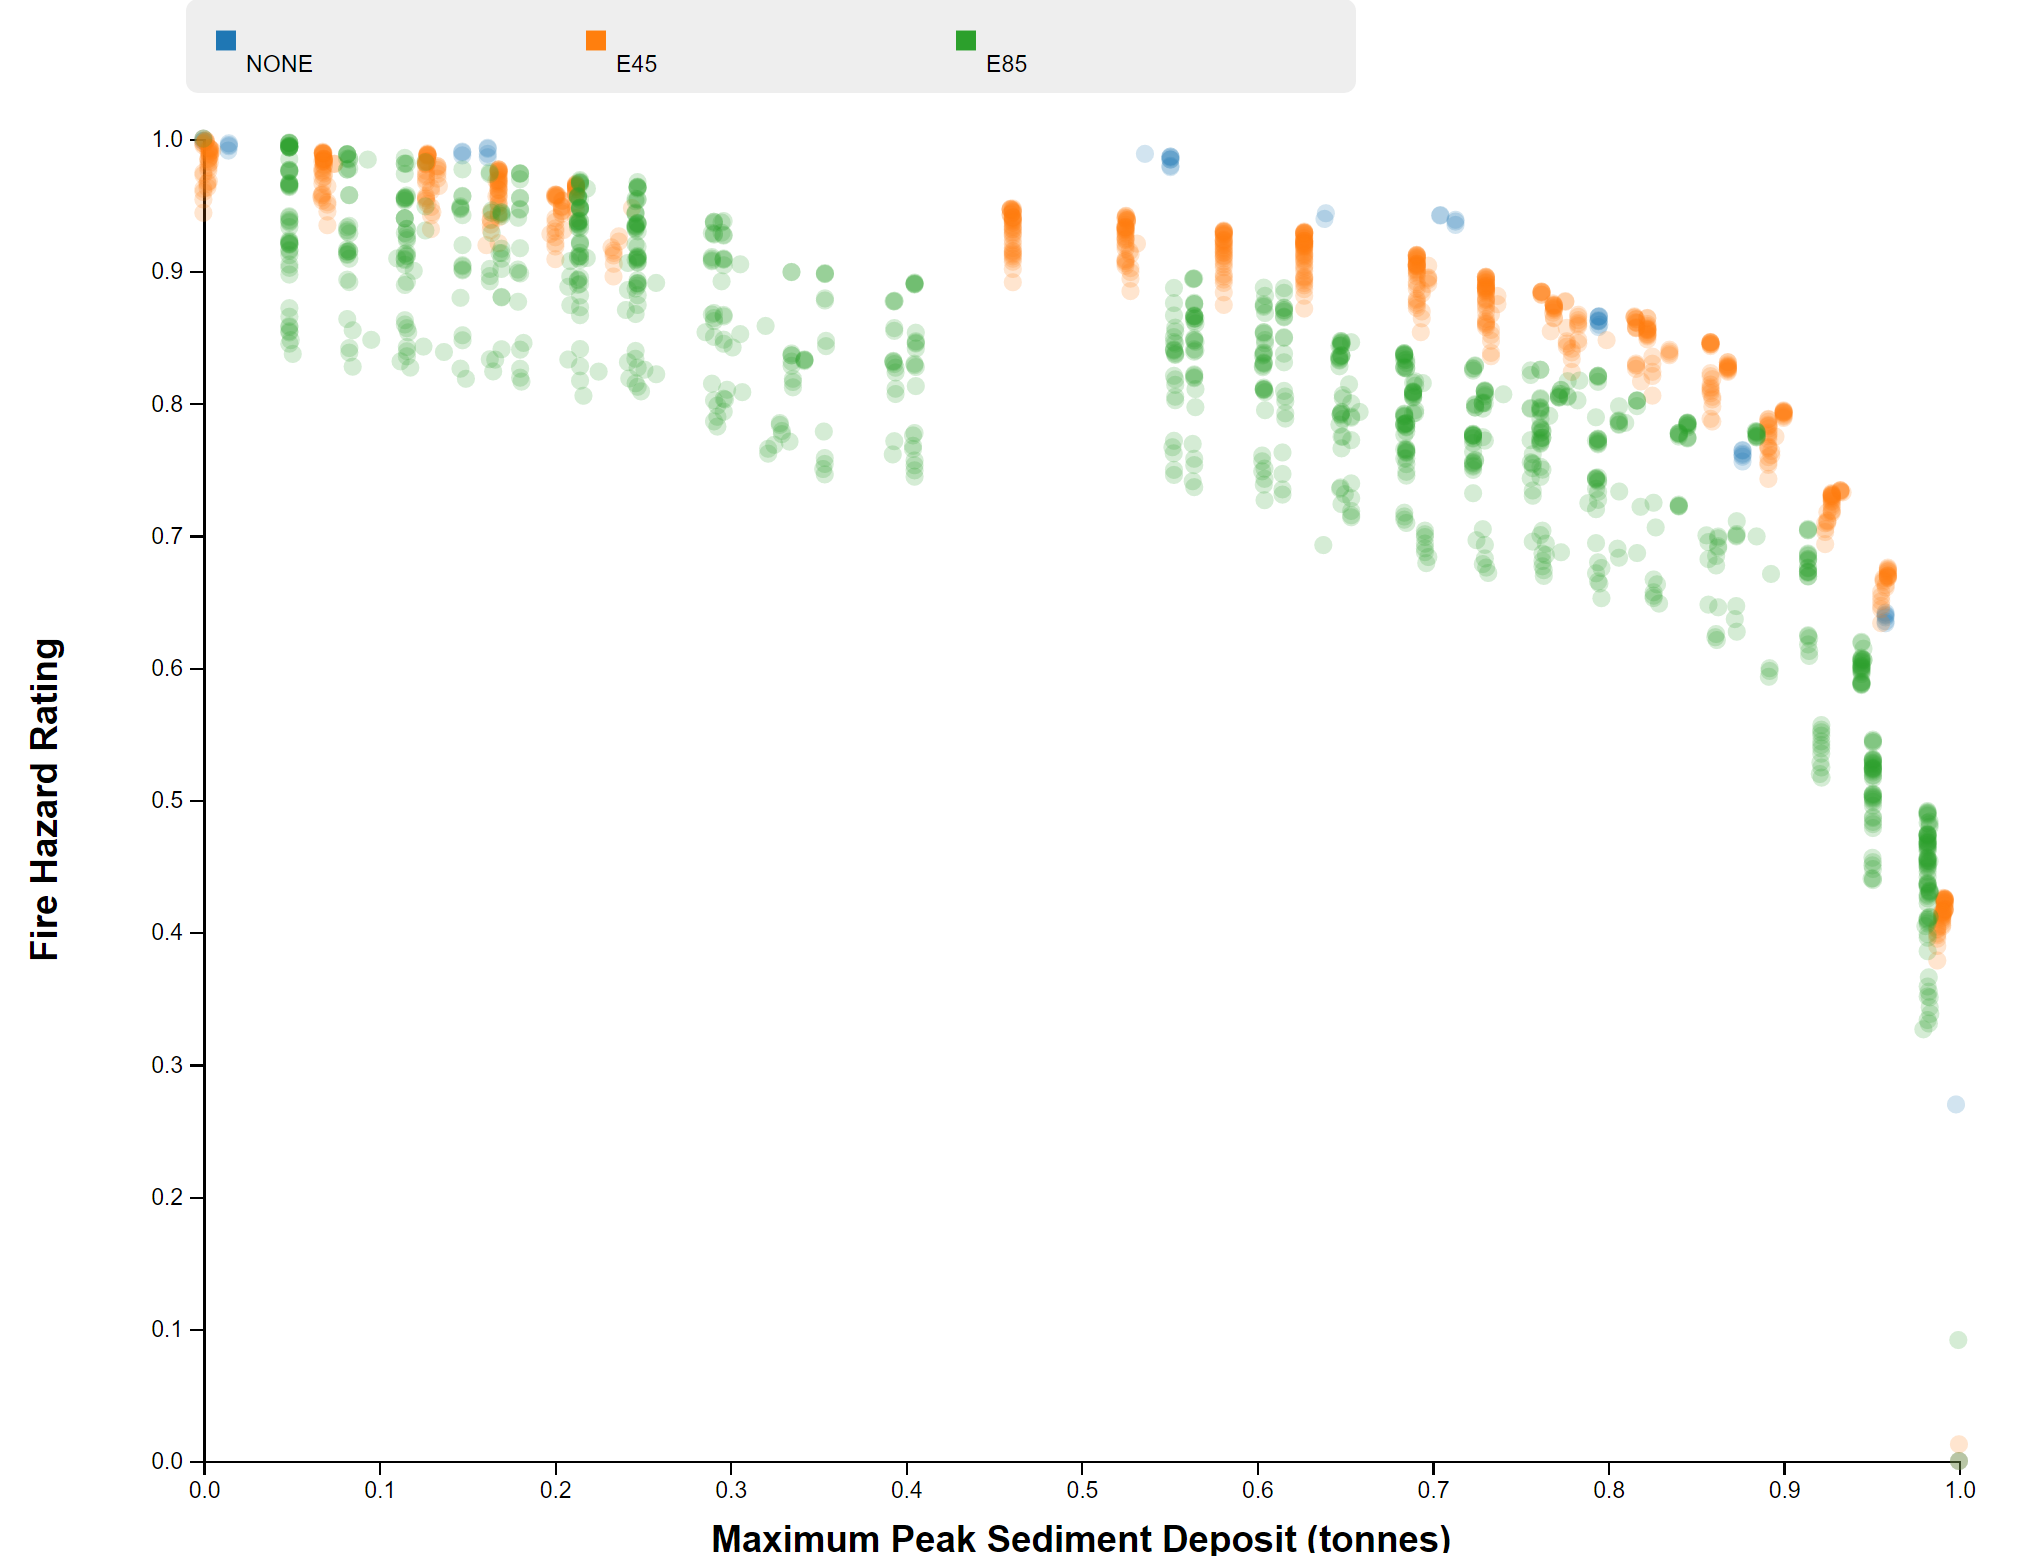
\includegraphics[width=.75\textwidth]{../images/2DSlice_Sed_Fire}
\caption[Sediment delivery vs. fire hazard for all climate scenarios]{Sediment delivery versus fire hazard for all climate scenarios.}
\label{fig:pairplotSedFire}
\end{figure}

\begin{table}[]
\centering
\caption[Sediment delivery-fire hazard conflict across climate scenarios]{Conflict between sediment delivery and fire hazard across climate scenarios.}
\label{tab:pairConflict-SedFire}
\begin{tabular}{llll}
\textbf{}     & \textbf{$C_{ij}$} & \textbf{$c_{ij,\rho}$} & \textbf{$c_{ij,d}$} \\ \hline
\textbf{None} & 0.36039           & 0.9927                 & 0.3630              \\
\textbf{E45}  & 0.36097           & 0.9853                 & 0.3664              \\
\textbf{E85}  & 0.38261           & 0.9514                 & 0.4021
\end{tabular}
\end{table}

\section{Discussion}
We divide our discussion of results into three sections: first, the decreasing provision of individual ecosystem services with climate change; second, the increase in the number of solutions; and third, conflict and the joint provision of ecosystem services.

\subsection{Decreasing provision of individual ecosystem services}
We observe decreasing provision of individual ecosystem services with increasing severity of climate change. In particular, we see that the difference between no climate change (None) and mild climate change (E45) was greater than the difference between mild climate change (E45) and severe climate change (E85). Refer to Table \ref{tab:frontiersSummary}. This suggests that, at least for the ecosystem services in this study, the realization of climate change is more significant than the severity of that change.

\paragraph{Sediment delivery}
Investigating the cause of the degradation in sediment delivery, we find that the average spike in sediment delivered as a result of performing a fuels treatment increases with climate change. See Figure \ref{fig:avgSedimentDelivery}. The average sediment delivery per fuel removal under E45 is nearly twice the sediment delivery under the None scenario (81\% higher), and the E85 scenario is 0.4\% higher than that. This is driven by two underlying factors: the response in sediment delivery to prescribed burns and the frequency with which prescribed burns are assigned\footnote{For additional information on how treatment units are assigned a specific fuel removal technique such as thinning or prescribed burn, see the appendix, \S \ref{chap:appendix_drinkTreatments}.}. Our simulations show that increasing the severity of climate change causes pronounced increases in sediment delivery as a result of prescribed burns. We also find that relative to the None scenario, prescribed burns are assigned more frequently in the climate change scenarios -- 8 times more frequently in E45 and 10.1 times more frequently in E85. See Table \ref{tab:prscBurnsInClimChange}. These effects combine to produce the result seen in Figure \ref{fig:avgSedimentDelivery} of sediment delivery levels that increase with climate change severity.

\begin{figure}[ht]
\centering
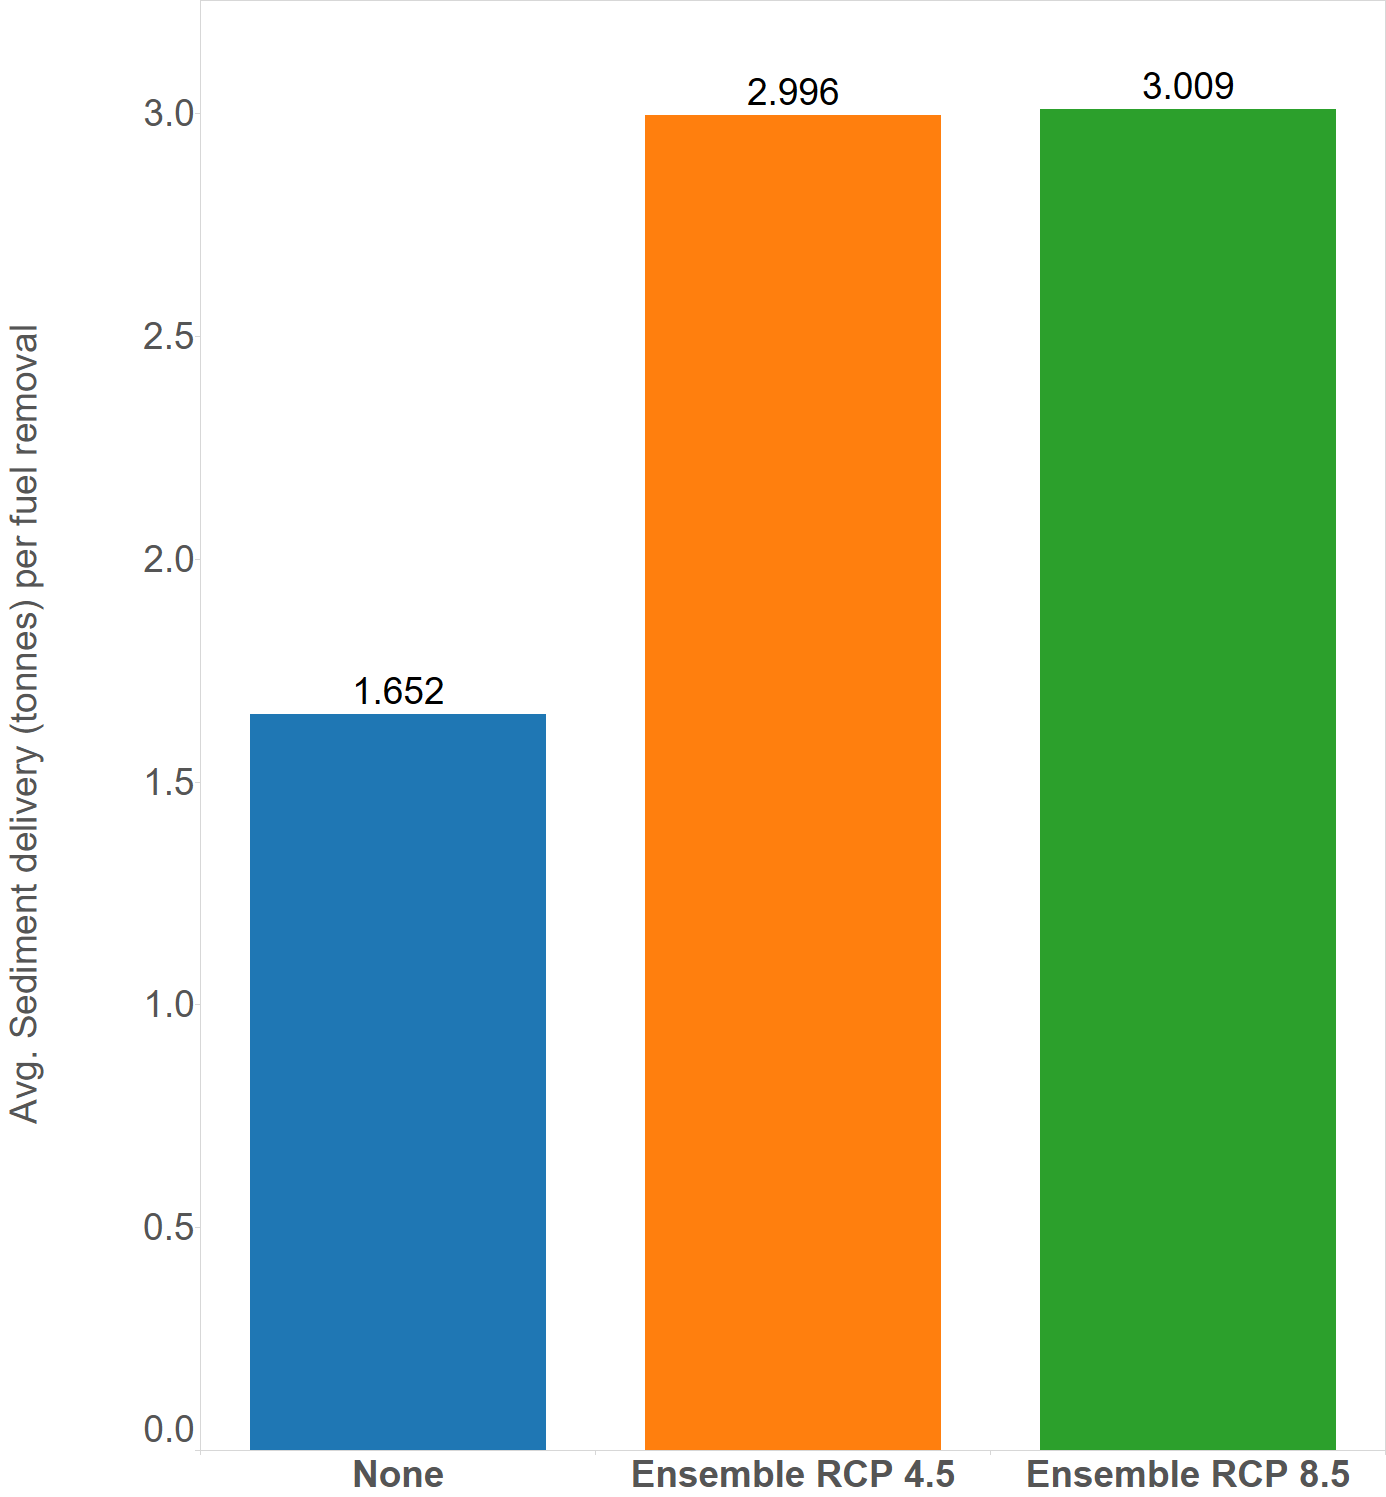
\includegraphics[width=.55\textwidth]{../images/AvgSedimentSpikes}
\caption[Average sediment delivery across climate scenarios]{Average spike in sediment delivery as a result of performing fuel removals for each climate change scenario.}
\label{fig:avgSedimentDelivery}
\end{figure}

\begin{table}[]
\centering
\caption[Frequency and impact of prescribed burns across climate scenarios]{Frequency and impact of prescribed burns for each climate scenario. The combination of more frequent prescribed burns and increased sediment delivery per prescribed burn results in the higher values of sediment delivery in E45 and E85 observed in Figure \ref{fig:avgSedimentDelivery}.}
\label{tab:prscBurnsInClimChange}
\begin{tabular}{llll}
                                                                                                           & \textbf{None} & \textbf{E45} & \textbf{E85} \\ \hline
\textbf{\begin{tabular}[c]{@{}l@{}}Average sediment delivery\\ (tonnes) from prescribed burn\end{tabular}} & 31.23            & 48.56          & 48.97          \\
\textbf{\begin{tabular}[c]{@{}l@{}}Number of prescribed\\ burns assigned\end{tabular}}                     & 34         & 272        & 344       
\end{tabular}
\end{table}

\paragraph{Fire hazard}
For the fire hazard objective, recall that we constrain the total area treated in each period. We first note that the increase in fire hazard with climate change severity is not simply due to the model selecting less area for treatment. Across both treatment periods and all climate scenarios, the model consistently utilizes over 99\% of the allowable value -- see Table \ref{tab:treatedAreas}. Instead, we find that the increase in fire hazard is due to the impact of climate change on the fuel model classification of the treatment units in the Drink Area. In E45 and E85, more treatment units are assigned a fuel model classification that is associated with higher fire hazard (refer to Table \ref{tab:firehazards} for the mapping from fuel models to fire hazard). This is shown in Figure \ref{fig:distOfFireHazards}, where we observe a larger percentage of treatment units having a fire hazard rating of either 4 or 5 under the E45 and E85 scenarios than in None.

\begin{table}[]
\centering
\caption[Area treated per period across climate scenarios]{Areas treated per period across climate scenarios. The values are nearly constant for both periods and for each climate scenario.}
\label{tab:treatedAreas}
\begin{tabular}{llll}
                                                                                                           & \textbf{None} & \textbf{E45} & \textbf{E85} \\ \hline
\textbf{Area treated (ha) in period 1} & 2427.31            & 2426.90 & 2414.58          \\
\textbf{Area treated (ha) in period 2}                     & 2427.56         & 2427.71        & 2427.63      
\end{tabular}
\end{table}

\begin{figure}[ht]
\centering
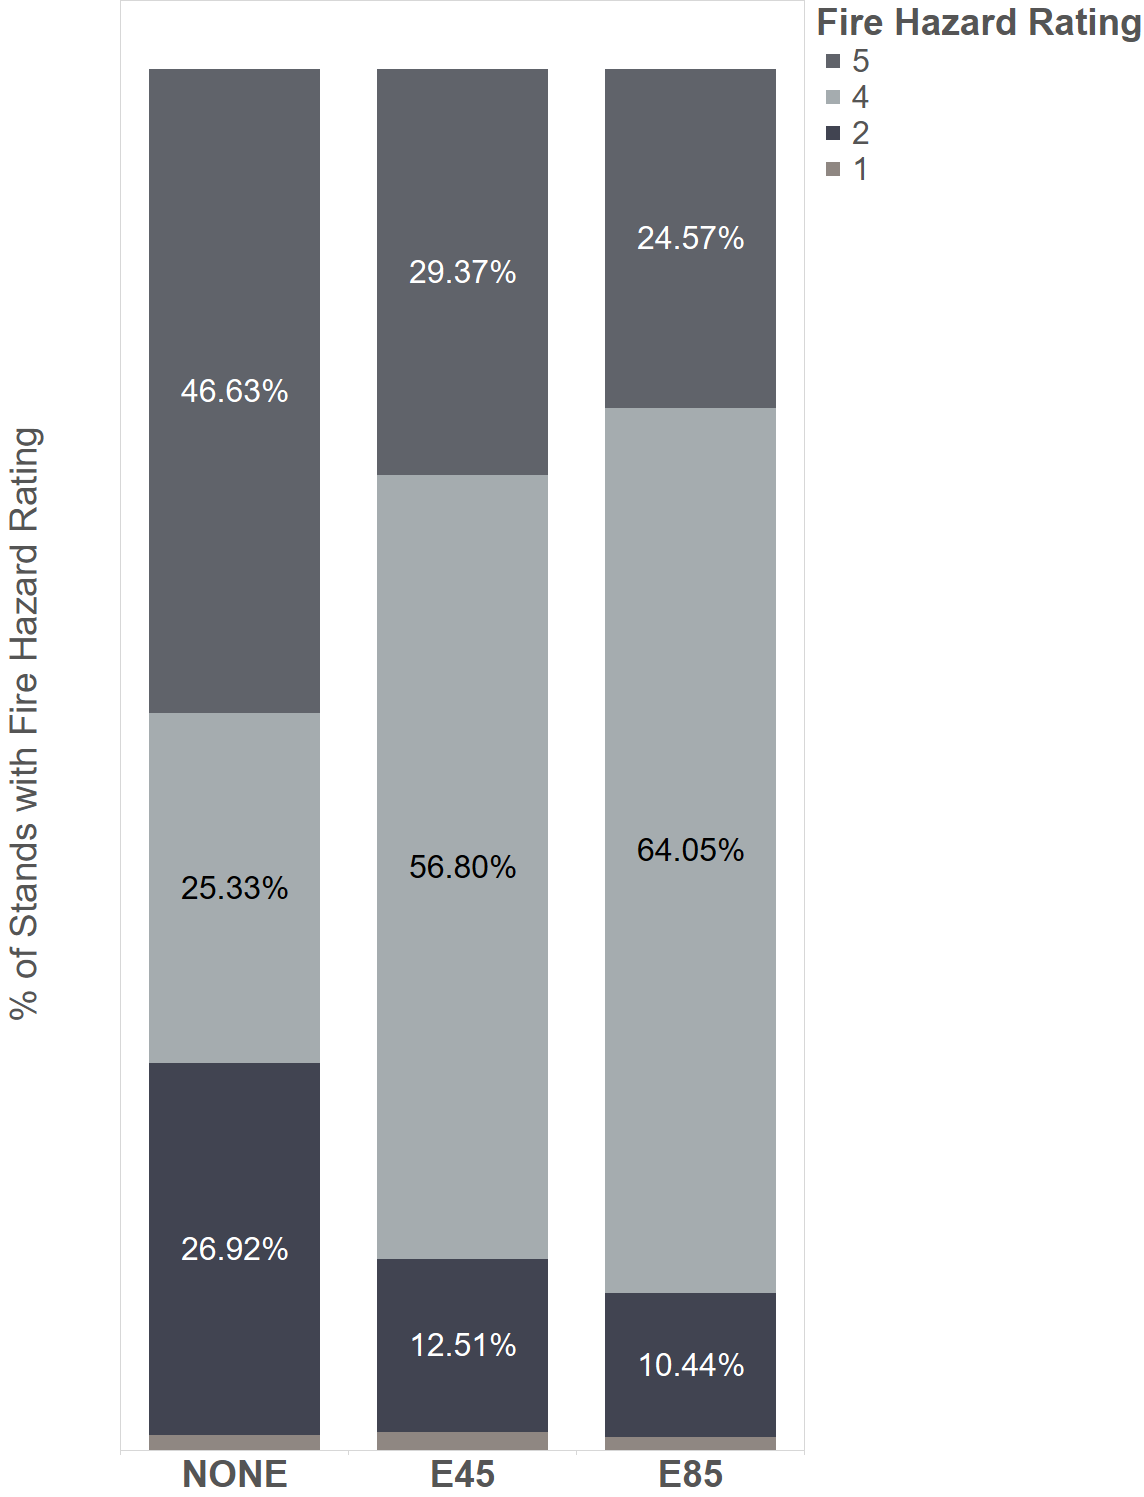
\includegraphics[width=.5\textwidth]{../images/FireHazardRatingsPerClimateScenario}
\caption[Distribution of fire hazard ratings over the Drink Area for each climate change scenario]{Distributions of fire hazard ratings across the Drink Area under each climate change scenario. Moving from left to right (in increasing climate change severity), we observe an increase in the percent of treatment units classified with more extreme fire hazards (ratings of 4 and 5).}
\label{fig:distOfFireHazards}
\end{figure}
% If we need a map, show a single map that shows the diff in FH at 2095 for a good sol from E85 - good sol from None

\paragraph{NSO habitat}
Lastly, we find that the decrease in NSO habitat is largely due to the effects of climate change on the vegetation in the Drink Area. Recall that of the criteria used to determine if a treatment unit qualifies as NSO habitat, two are determined by vegetation characteristics: the presence of at least one tree with DBH $> 76$ cm and canopy closure of at least 60\%. While climate change has minimal impact on the former, the average canopy closure for treatment units in the Drink Area decreases with increasing severity of climate change. See Figure \ref{fig:canopyClosure}.

\begin{figure}[ht]
\centering
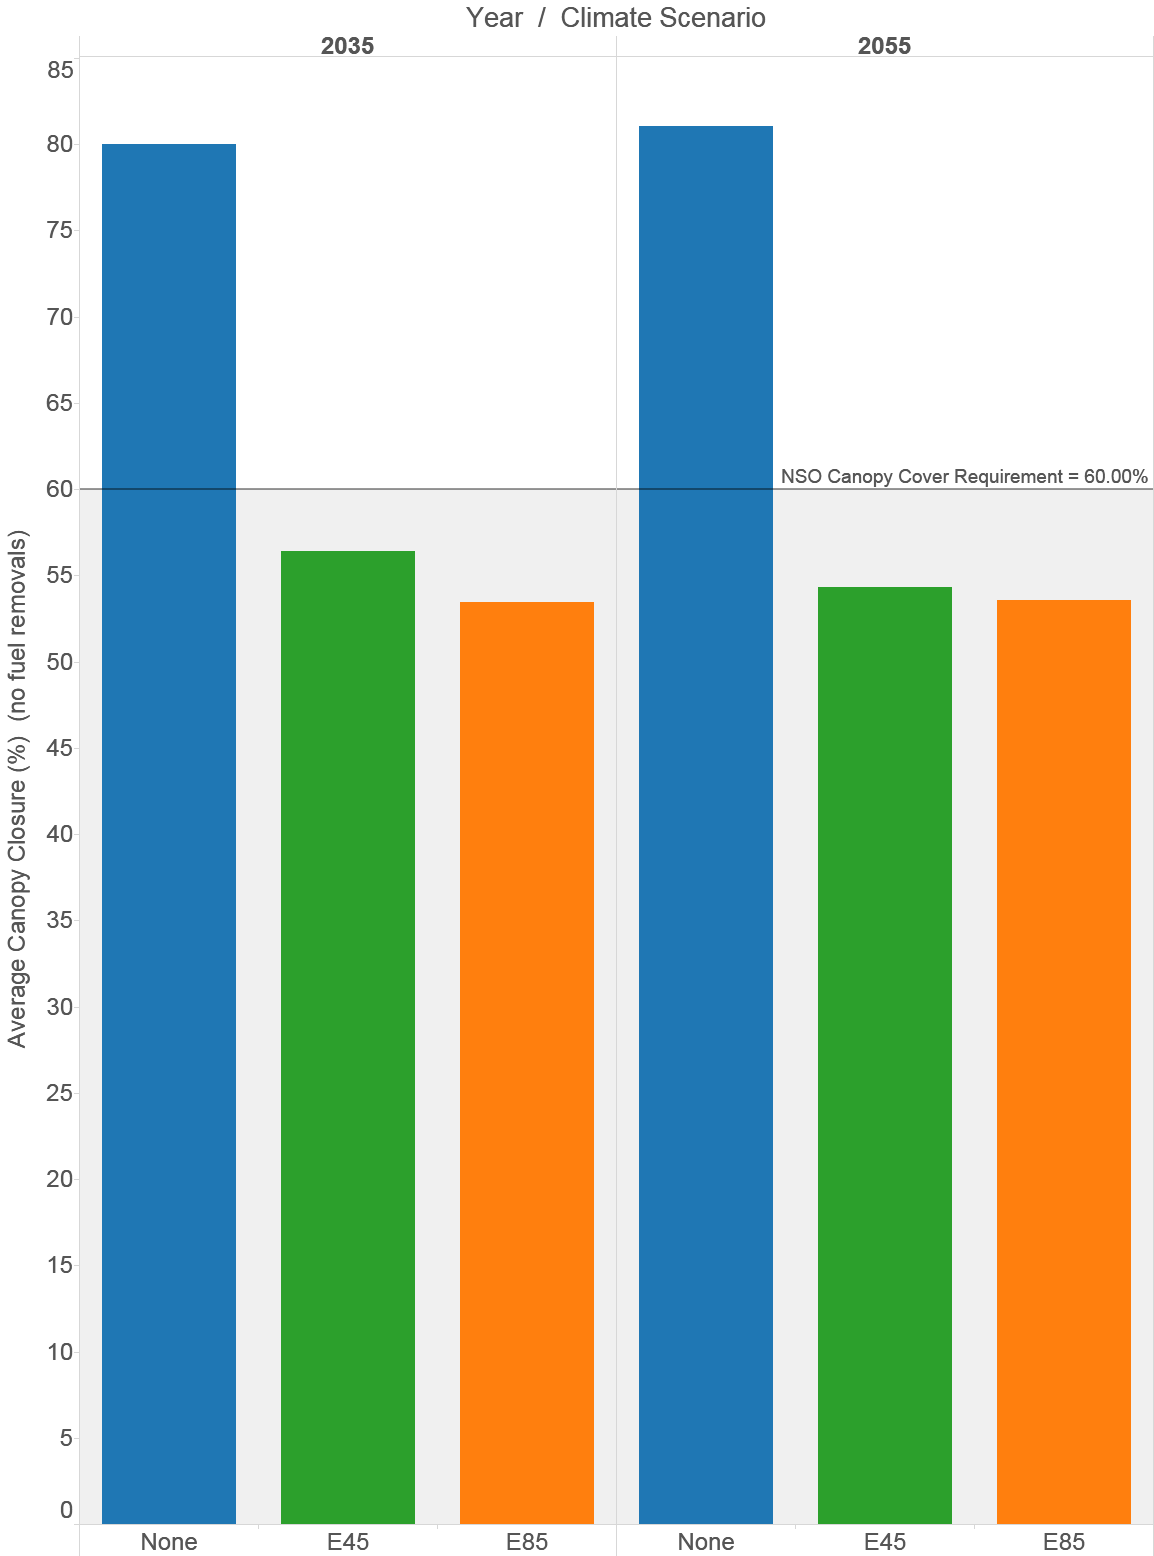
\includegraphics[width=.5\textwidth]{../images/AvgCanopyCover_NoTrtmts}
\caption[Average canopy closure in the Drink Area across climate scenarios]{Average canopy closure for treatment units in the Drink Area for each climate scenario. Shown are canopy closure values during years 2035 and 2055 (the years in which NSO habitat is measured) when no fuel removals are performed. We see that with increasing climate change severity, canopy closure decreases.}
\label{fig:canopyClosure}
\end{figure}


\subsection{Variation in number of solutions}
With increasing climate change severity, we noted an increase in the number of solutions generated by our model:  51 for $Z_{\text{None}}$, 701 for $Z_{\text{E45}}$, and 1083 for $Z_{\text{E85}}$. We suspect this is because fuel removals more frequently alter whether a treatment unit qualifies as NSO habitat in the climate change scenarios. This also drives the greater variation in NSO habitat seen for the E45 and E85 scenarios.

The number of instances in which performing a fuel removal disqualifies a treatment unit from being NSO habitat is 24 in None, 63 in E45, and 67 in E85. Let us refer to such fuel removals as ``disqualifying treatments.'' By more than doubling the number of disqualifying treatments in the E45 and E85 scenarios, additional solutions are produced in those frontiers. If these disqualifying treatments generated little fire hazard reduction in return for the disqualification of NSO habitat, then these decisions would not be part of the optimal solutions $\mathbf{x} \in P$. However, we find that the reduction in fire hazard for a given disqualifying treatment increases with climate severity (Figure \ref{fig:nsoHabDQFHEfficacy}). This leads to greater incentive for the model to sacrifice NSO habitat in favor of fire hazard reduction.

\begin{figure}[ht]
\centering
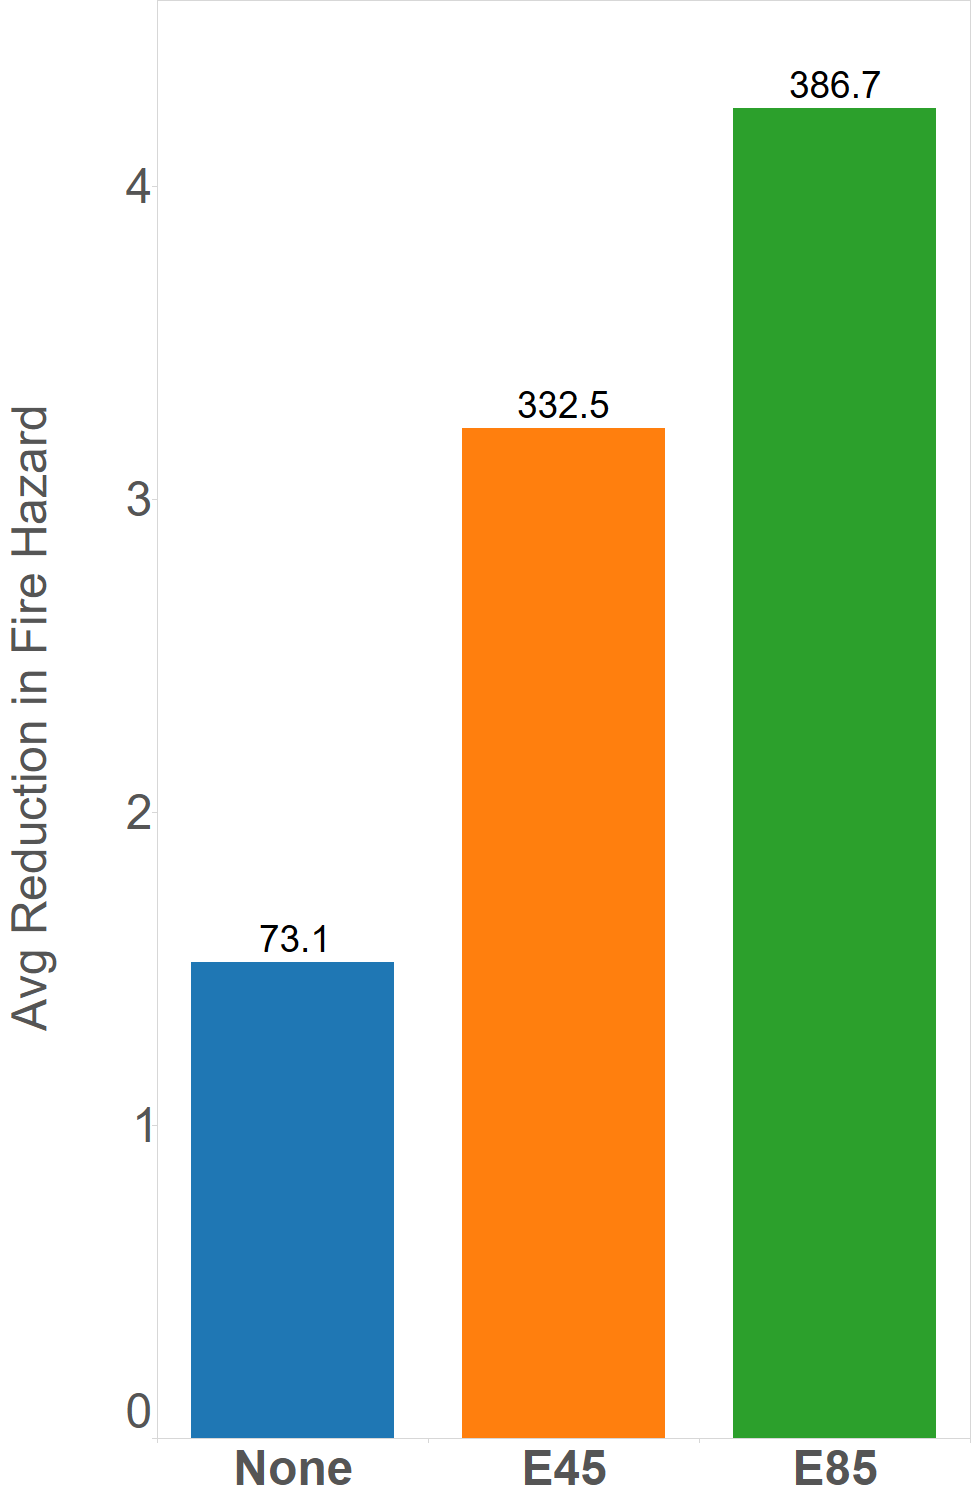
\includegraphics[width=.5\textwidth]{../images/AvgFireHazardEffectivenessForNSODQs}
\caption[Efficacy of fuel removals for NSO habitat disqualification]{Some treatment units may always be NSO habitat and others may never be NSO habitat, regardless of model decisions. For those treatment units which vary based on model decisions, we see here the average efficacy of fuel removals which disqualify their being NSO habitat. This value increases with increasing climate change, indicating greater incentive for the model to forgo NSO habitat in favor of fire hazard reduction.}
\label{fig:nsoHabDQFHEfficacy}
\end{figure}

Together, these factors lead to an increase in the number of solutions as well as greater variation in the total amount of NSO habitat provided by the models.

\subsection{Conflict and the joint provision of ecosystem services}
We observe a decreasing hypervolume with increasing climate change severity. Lower values for the hypervolume are indicative of more conflict, meaning that climate change induces more conflict among the ecosystem services and leads to less joint provision of objectives.

The difference in hypervolume between None and E45 $I_{H1}(Z_\text{None}) - I_{H1}(Z_\text{E45}) \approx 0.01$. Recall that a difference of $h$ in hypervolumes equates to a difference of $h^{1/M}$ in each objective (Figure \ref{fig:Hypervol10percent}). Thus, despite the small size of the difference between $I_{H1}(Z_\text{None})$ and $I_{H1}(Z_\text{E45})$, the additional volume of the objective space bound by None signifies an additional joint provision of objectives of approximately 21.6\%. This difference means that there are solutions in None that represent an simultaneous improvement in each objective of more than 7\% over any solution in E45.  The difference in hypervolume indicators is greater between None and E85, approximately 0.05. This represents an additional joint provision of ecosystem services of approximately 36.2\% in None compared to E85, or an improvement in each objective of more than 12\%.

From the hypervolumes alone, it is uncertain whether None represents a strictly better frontier than either E45 or E85 or if, despite their smaller hypervolume values, E45 and E85 enclose some region of the objective space that is not enclosed by None. Any such region would extend further into the objective space, representing the presence of solutions that achieve greater joint provision of ecosystem services. The results of the binary hypervolume were presented in Table \ref{tab:binaryHypervols}.

The results show that no frontier is dominated by any other, and each frontier encloses some region of the objective space not enclosed by the others. For the pairs of frontiers for which the binary hypervolume is greatest ($(Z_\text{None},Z_\text{E85})$ and $(Z_\text{E45},Z_\text{E85})$), this additional extension into the objective space is most obvious in Figure \ref{fig:pairplotSedFire}. We see for values of sediment delivery between 0.15 and 0.8 that None appears to dominate E45 which appears to dominate E85. Further, for sediment delivery values between 0.8 and 1, it appears that E45 dominates E85 and None, between which any domination relationship is difficult to discern.

The existence of these areas leads to the lower value of conflict $C_{ij}$ between sediment delivery and fire hazard in None and E45 than in E85. We claim that this is a success of the conflict metric $C_{ij}$: all frontiers in the sediment delivery-fire hazard plane of Figure \ref{fig:pairplotSedFire} are similar. They have similar shape and achievement towards the sub-dimensional ideal solution, yet the metric is able to distinguish differences in conflict between them.

For the other pairwise objective comparisons, as we saw in Figures \ref{fig:pairplotNSOSed} and \ref{fig:pairplotNSOFire}, the distribution of solutions more closely resembles a uniform two-dimensional scattering. There is no clear conflict pattern between them similar to what we saw in Figure \ref{fig:pairplotSedFire}. As a result, $C_{ij}$ reports little conflict between these objective pairs. However it varied in unexpected ways between the climate scenarios. In these cases, we find that the distance component $c_{ij,d}$ was primarily responsible for the variations, as the rank correlations tended to be insignificantly different from 0.5. It appears the conflict metric $C_{ij}$ is susceptible to such variations when neither the $c_{ij,d}$ nor $c_{ij,\rho}$ component tends towards their limiting values of 0 and 1.

% In general, however, it was really awesome.
However, in general, we find our process of utilizing the hypervolume measures and the proposed conflict metric to have been successful in quantifying conflict within and among the frontiers. The pairwise conflict metric successfully identified the pair of objectives which demonstrated the most conflict, and the hypervolumes indicated which climate scenarios allow for greater joint provision of ecosystem services.

\section{Management implications}
The management implications of the findings of this case study largely entail required adaptations to climate change. The degradation in the individual and joint provision of ecosystem services means that the decision makers for the Drink Area may need reevaluate the priorities given to these objectives. For instance, because in the case of climate change a given reduction in fire hazard requires a more substantial sediment delivery, forest managers may need to consider which of these objectives they are more comfortable compromising. Status quos will change, such as performing fire hazard reduction techniques and being comfortable with the resulting impacts on NSO habitat or watershed sediment content. Under climate change, we saw that fuel removal techniques are predicted to be simultaneously more intensive and less effective. If there are thresholds for the allowable levels of sediment delivery or NSO habitat, those may need to be revisited in light of the increased fire hazard required to exist within those thresholds.

Managers will benefit from an awareness of how the conflict among objectives is changing. Again, it allows them to reevaluate current thresholds on objectives and determine if those values are still sensible. It also may force managers to consider their objectives again and determine if some hold a higher priority than others. For instance, if sediment delivery and fire hazard become increasingly incompatible, which should be subject to a greater sacrifice in order to maintain more of the other? Further, while undiscussed here, each solution to these models captures a management plan, complete with the spatio-temporal information regarding fuel removals. By identifying similarities in management plans relative to a given objective achievement, it allows managers to identify which fuel removal practices are most robust across the climate scenarios. Similarly, it allows them to identify which fuel removal practices are least desired, resulting in an objective achievement deemed too poor for practical implementation.